%\linenumbers*
\chapter{DESCRIPTIONS OF DATA, MODELS AND METHODS}
\label{sec:SIMULATIONDATAMODELSANDMETHODS}

\section{Data}
\label{sec:Data}

All of the datasets used here for climate analyses, model parametrizations and
erosion simulations are obtained from the South Downs, England, UK (Figure
\ref{fig:DailyRainfallDataSite}).
One of the reasons for choosing this particular site is, because the area has
been extensively monitored for soil erosion since the late 1970s
\citep{boardman1995-177,boardman2003-176}, that data availability of the
site is reasonably great. In addition, there is a well-established expertise
about the area that can be referenced to the current research
\citep{boardman1995-177,favis-mortlock1995-365,favis-mortlock1997-79,
favis-mortlock1998-141,boardman2001-346,boardman2003-176}.

\subsection{Rainfall Data}
\label{sec:RainfallData}

Reported mean annual rainfall of the South Downs, UK is between 750 and 1000 mm
with an autumn peak \citep{potts1983-88}. Mean annual temperature is
9.8\textcelsius\ with a January mean of 3.9\textcelsius\ and a July mean of
16.3\textcelsius\ \citep{potts1983-88}.

Three temporally and spatially different observational rainfall datasets were
acquired from the site (Table
\ref{tab:PrecipitationDataUsedForCurrentRainfallTrendInvestigation}).

Observed monthly 0.5\textdegree$\times$0.5\textdegree\ grid rainfall data (CRU
TS 2.0---0.5\textdegree$\times$0.5\textdegree\ Gridded Monthly Climate Data for
Land Areas) for 100 years were obtained from \citet{mitchell2004-a}. Coordinates
of the centre point of the study grid are 50.75\textdegree\ (Latitude) and
-0.25\textdegree\ (Longitude).

\begin{table}[htbp]
  \figureversion{tabular}
  \centering
  \caption{Precipitation data used in this study}
  \label{tab:PrecipitationDataUsedForCurrentRainfallTrendInvestigation}
  \small
    \begin{tabular}{cccc}
    \toprule
    \textbf{Temporal Scale} & \textbf{Spatial Scale} &
\textbf{Duration} & \textbf{Studied Rainfall Characteristics}\\
    \midrule
    month & 0.5\textdegree$\times$0.5\textdegree\ grid & 100 years
&amount\\
    day & 11 stations & 10--99 years & 7 indicators (see Table
\ref{tab:RainfallIntensityIndicators})\\
    event$^\dagger$ & 3 stations & 2--13 years & amount, duration,
intensity\\
    \bottomrule
%   \addlinespace[1mm]
    \multicolumn{4}{p{10cm}}{\footnotesize $^\dagger$ Aggregated
1-min data originally from tipping bucket data}
    \end{tabular}
\end{table}

Daily rainfall amounts from 11 stations were obtained for the period of 1904 to
2004. Data durations are varied for each station (Table
\ref{tab:DetailsOfDataStations}). Locations of individual daily stations are
shown in Figure \ref{fig:DailyRainfallDataSite}.

\begin{figure}[phtb]
  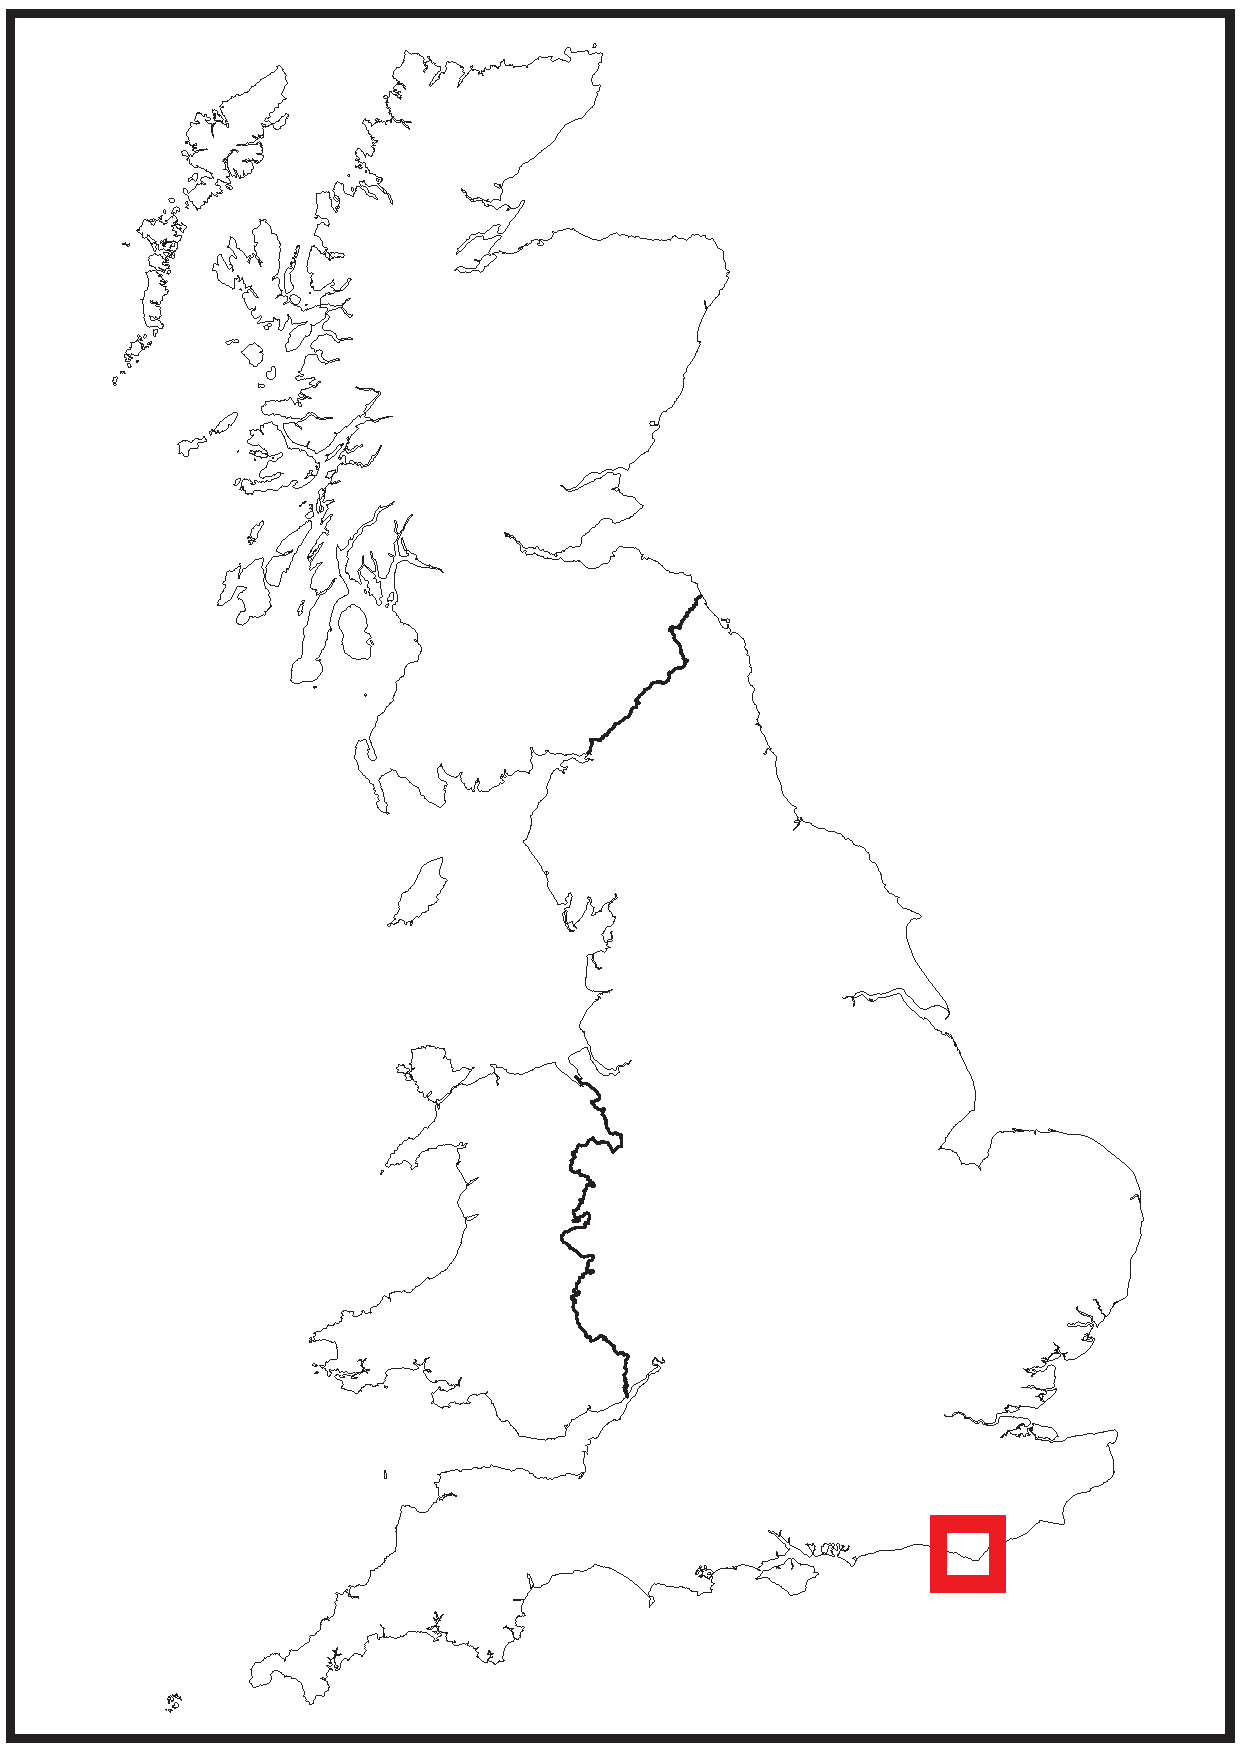
\includegraphics[width=0.19\textwidth]{./img/ukoutline}
  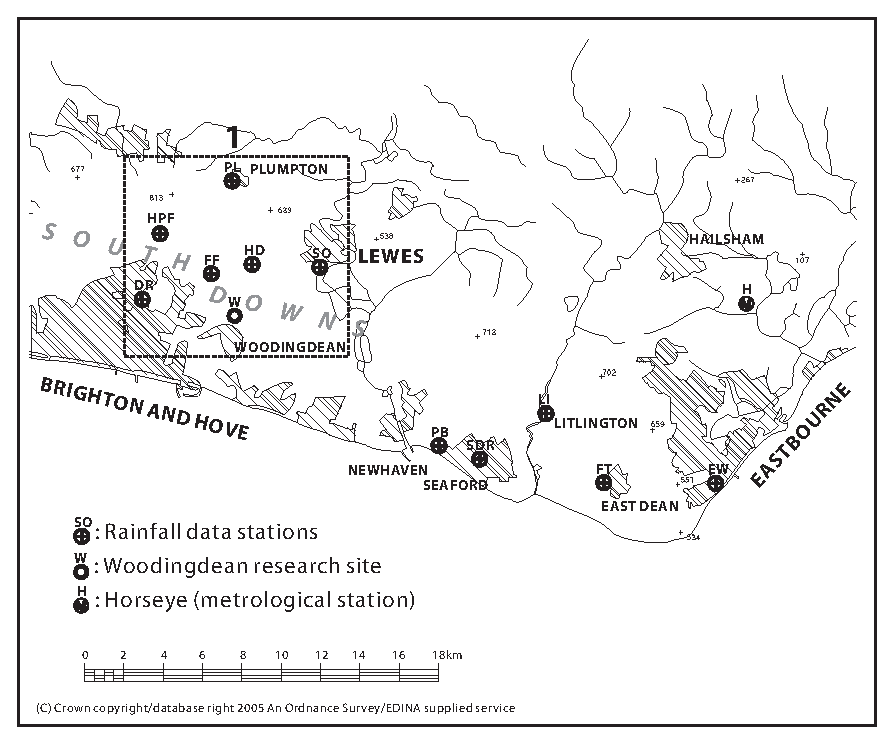
\includegraphics[width=0.8\textwidth]{./img/dailydatasite}
  \caption[Locations of daily rainfall data stations]{Locations of daily
rainfall data stations. DR: Ditchling Road, SO: Southover, PL: Plumpton, SDR:
Seaford D. Road, EW: Eastbourne Wilm., FT: Friston Tower, LI: Litlington, PB:
Poverty Bottom, HPF: High Park Farm, HD: Housedean, FF: Falmer Farm, W:
Woodingdean (soil, slope, crop management), H: Horseye (temperature);
\emph{dotted frame(1)} indicates the area shown in Figure
\ref{fig:EventRainfallDataSite}.}
  \label{fig:DailyRainfallDataSite}
\end{figure}

High resolution event rainfall data measured by tipping-bucket gauges were
obtained from three stations---Ditchling Road, Southover and Plumpton---nearby
the research site (Figure \ref{fig:EventRainfallDataSite}). Detection limit of
the tipping bucket was 0.2 mm. Data duration from each station ranged from 2 to
13 years with some missing data between 1995 and 1998. This might have been
because of vandalisms in the area, a defunct station or temporary gauge
malfunctions (personal communications with Environment Agency on 1 March 2003).
It should be noted that there are only a few rainfall stations which record
event rainfall in the study region (Figure \ref{fig:EventRainfallDataSite}).
Long term high resolution rainfall data with good quality is seldom available
because of, for example, a large size of data file. However, quality of the data
used here was reasonably good of capturing rainfall intensity details.

\begin{figure}[phtb]
  \centering
  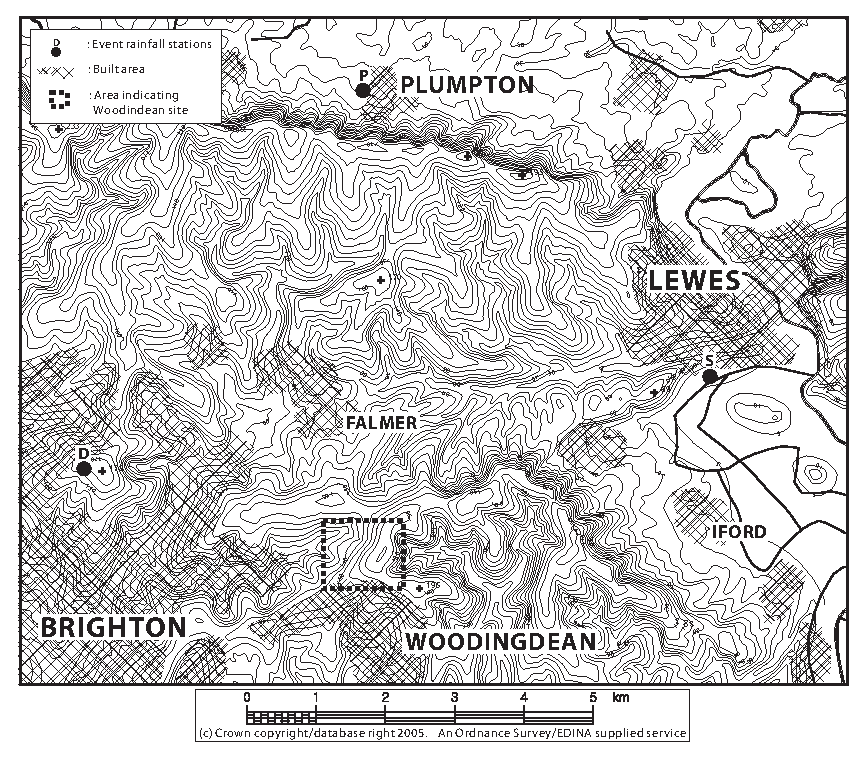
\includegraphics[width=0.8\textwidth]{./img/eventdatasite}
  \caption[Locations of event rainfall data stations]{Locations of event
rainfall data stations. \emph{filled circles}: event rainfall data stations (S:
Southover, D: Ditchling Road, P: Plumpton); Woodingdean site is indicated by
\emph{dotted frame} (see Figure \ref{fig:WoodingdeanSite} for the detail)}
  \label{fig:EventRainfallDataSite}
\end{figure}

The detailed information about the daily and event data are summarised in Table
\ref{tab:DetailsOfDataStations}.

\begin{table}[htbp]
  \figureversion{tabular}
  \centering
  \caption{Details of rainfall data stations}
  \label{tab:DetailsOfDataStations}
    \small
    \begin{tabular}{lllll}
      \toprule
      \textbf{Code} & \textbf{Station} & \textbf{Data type} &
\textbf{Grid reference} & \textbf{Periods}\\
      \midrule
      DR & Ditchling Road & daily & TQ314076 & 1980--1989\\
      SO & Southover & daily & TQ407093 & 1980--1998\\
      PL & Plumpton & daily & TQ356136 & 1980--2000\\
      SDR & Seaford D. Road & daily & TV491993 & 1980--2000\\
      EW & Eastbourne Wilm. & daily & TV611980 & 1980--2000\\
      FT & Friston Tower & daily & TV551982 & 1980--2000\\
      LI & Litlington & daily & TQ523020 & 1980--2000\\
      PB & Poverty Bottom & daily & TQ467002 & 1980--2000\\
      HPF & High Park Farm & daily & TQ331115 & 1974--2004\\
      HD & Housedean & daily & TQ369093 & 1967--2004\\
      FF & Falmer Farm & daily & TQ342084 & 1904--2002\\
      S & Southover & event & TQ407093 &
1993--2001$^\dagger$\\
      D & Ditchling Road & event & TQ315077 &
1991--2003$^\ddagger$\\
      P & Plumpton & event & TQ357135 & 2000--2002\\
      \bottomrule
%     \addlinespace[1mm]
      \multicolumn{5}{l}{\footnotesize $^\dagger$  with
missing data between Sep. 1996 to Jun. 1998}\\
      \multicolumn{5}{l}{\footnotesize $^\ddagger$  with
missing data between Feb. 1995 to Sep. 1997}
    \end{tabular}
\end{table}

\subsection{Other Data}
\label{sec:OtherData}

\subsubsection{Soil}
\label{sec:Soil}

Other input data, such as soil properties and slope profiles, were either
directly acquired from previous studies \citep{favis-mortlock1998-141} or
calibrated as shown in Table \ref{tab:HydrologicalAndErosionalParameters}.
Unless it was critically necessary, all the data were kept unchanged. This
minimizes unknown effects which may occur because of changing other erosional
factors, and also permits the present research to concentrate on the effect of
rainfall intensity changes.

The erosion simulation site is 7.7 ha in size, and is located at Drove Road,
Woodingdean (NGR: TQ358069): this is in the UK South Downs, about 6 km southwest
of Lewes (Figure \ref{fig:WoodingdeanSite}). Soil, slope and crop management
details are obtained from this site.

\begin{figure}[phtb]
  \centering
    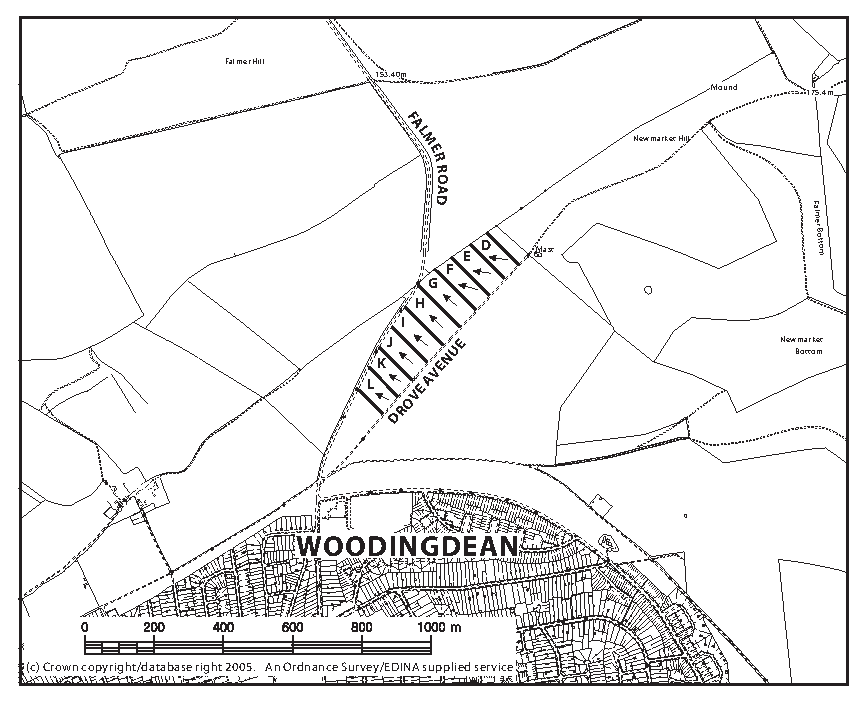
\includegraphics[width=0.8\textwidth]{./img/woodingdean}
  \caption[Woodingdean site]{Woodingdean site. The arrows indicate
approximate downslope direction. Each letter (D-L) denotes hillslope profiles
used for model simulations.}
  \label{fig:WoodingdeanSite}
\end{figure}

The soil in the area is shallow (around 20 cm to chalk) and stony silty rendzina
of the Andover series \citep{jarvis1984-soils}. The Andover silt loams of the
South Downs are both stony and prone to crusting. All the soil input parameters
are summarised in Table \ref{tab:AndoverSoilDetails} and Table
\ref{tab:HydrologicalAndErosionalParameters}.

\begin{table}[htbp]
  \figureversion{tabular}
  \centering
  \caption[Andover soil details]{Andover soil details
\citep[From][]{favis-mortlock1998-141}}
  \label{tab:AndoverSoilDetails}
    \small
    \begin{tabular}{lrrrr}\toprule
    & \multicolumn{4}{c}{Layer}\\
    \cmidrule{2-5}
    & \multicolumn{1}{c}{1} & \multicolumn{1}{c}{2} &
\multicolumn{1}{c}{3} & \multicolumn{1}{c}{4}\\
    \midrule
    Depth to bottom of layer (mm) & 150.0 & 200.0 & 300.0 & 1000.0\\
    Sand (\%) & 18.9 & 18.9 & 25.0 & 25.0\\
    Clay (\%) & 3.5 & 3.5 & 24.0 & 24.0\\
    Organic matter (\%) & 7.0 & 4.8 & 2.2 & 1.2\\
    Cation exchange capacity (meq/100 g of soil) & 45.0 & 39.0 &
30.0 & 14.0\\
    Coarse (Rock) fragments (\% vol) & 38.1 & 50.0 & 90.0 & 90.0\\
    \bottomrule
    \end{tabular}
\end{table}

Values for WEPP's parameters for effective hydraulic conductivity, together with
values for its three erodibility parameters, were subjectively adjusted
following the suggestions by \citet{favis-mortlock1998-141} (Table
\ref{tab:HydrologicalAndErosionalParameters}). The parameters for interrill and
rill erodibility ($K_i$ and $K_r$) were reduced, while the critical shear stress
parameter $\tau_c$ was increased. The value for the base line effective
hydraulic conductivity parameter $K_b$ was also increased. All the adjustments
were taken from \citet{favis-mortlock1998-141} with the exception of critical
shear stress parameter $\tau_c$ which was recalibrated to 6. This was done in
order to meet the recommended value of maximum  $\tau_c$ by the WEPP
documentation. All calibrated values were constrained to remain within the
recommended ranges in WEPP documentation \citep{flanagan1995-usda}.

\begin{table}[htbp]
  \figureversion{tabular}
  \centering
  \caption[Hydrological and erosional parameter values]{Hydrological and
erosional parameter values \citep[After][]{favis-mortlock1998-141}}
  \label{tab:HydrologicalAndErosionalParameters}
    \small
    \begin{tabular}{lrr}
    \toprule
    & Uncalibrated Hydrological & Calibrated Hydrological\\
    & and erosional parameters & and erosional parameters\\
    \midrule
    Effective hydraulic conductivity & &\\
    of top soil layer (mm/hr) & 2.1$^a$ & 3.0$^a$\\
    Interrill erodibility $K_i$ (kg s/m$^4$) & 5502700 & 2000000\\
    Rill erodibility $K_r$ (s/m) & 0.0871 & 0.0050\\
    Critical shear stress $\tau_c$ (N/m$^2$) & 3.5 & 6.0$^b$\\
    \bottomrule
%   \addlinespace[1mm]
    \multicolumn{3}{l}{\footnotesize $^a$ `baseline' effective
hydraulic conductivity for WEPP ($K_b$)}\\
    \multicolumn{3}{l}{\footnotesize $^b$ adjusted to 6 which is a
maximum value for cropland $\tau_c$}
    \end{tabular}
\end{table}

\subsubsection{Management}
\label{sec:Management}
A typical crop management practice for the area is continuous growing of winter
wheat. The typical timing of tillage operation for the area is shown in Table
\ref{tab:TillageOperationTiming}.

\begin{table}[htbp]
  \figureversion{tabular}
  \centering
  \caption[Tillage operation timing at Woodingdean site]{Tillage operation
timing at Woodingdean site \citep[From][]{favis-mortlock1998-141}}
  \label{tab:TillageOperationTiming}
    \small
    \begin{tabular}{lr@{ }l}
      \toprule
      \textbf{Operation} & \multicolumn{2}{l}{\textbf{Date}}\\
      \midrule
      Chisel plough & 20 & August\\
      Harrow & 15 & September\\
      Drill (Winter wheat) & 28 & September\\
      Roll & 1 & October\\
      Harvest & 29 & July\\
      \bottomrule
    \end{tabular}
\end{table}

\subsubsection{Topography}
\label{sec:TopographyData}
Slope angles in the site range from 12 to 20\%, with a convexity toward the
centre. The site was divided into nine sub-areas for modelling, approximately
down the line of greatest slope, which faces a northwesterly direction (Figure
\ref{fig:WoodingdeanSite}). The length of each slope varies from 125 to 180
metres, and width is 50 metres for all the slopes.

\subsubsection{Temperature}
\label{sec:Temperature}

Daily temperature records for 1990--2000 were obtained from Horseye Station
(NGR: TQ627083) (Figure \ref{fig:DailyRainfallDataSite}). The distance of this
station from the study site is about 25 km. This data set was used in this study
since no other data set was available from the region at that time. Average
annual maximum and minimum temperature are 14.9\textcelsius\ (SD:
5.5\textcelsius)\ and 6.6\textcelsius\ (SD: 4.9\textcelsius), respectively.

\section{Justification for Erosion Model Selection}
\label{sec:ModelConfiguration}

As the research aims to investigate impacts of extreme rainfall events, all soil
erosion models used in this research should be able to simulate a single erosion
event. WEPP, EUROSEM and RillGrow were chosen because of this reason. All three
models are capable of simulating single events while WEPP may also be used for
continuous simulations (Table \ref{tab:ModelsUsedInThePresentStudy}).

There are two more reasons why these models were used. One is that they use
different approaches to erosion simulations and rainfall intensity. WEPP, for
example, estimates soil erosion using steady-state approach
(Equation \ref{eq:weppsedimentload}) while EUROSEM employs a dynamic approach
using a mass balance equation (Equation \ref{eq:eurosemmassbalance}).
Both models also consider rill and interrill areas separately and use
different equations for describing processes in two areas. In terms of
rainfall intensity, WEPP uses rainfall intensity as effective rainfall
intensity for estimating interrill erosion. In EUROSEM rainfall intensity is
considered as a function of kinetic energy of raindrops which act as detachment
agents of soil particles.
RillGrow, on the other hand, is based on a
self-organising dynamic system to simulate the initiation and development of a
network of rills. RillGrow also does not consider rill and interrill areas
separately. All three models are described previously (Section
\ref{sec:SoilErosionPredictionModels}).
The other reason why these models were used is that they are
originally designed for different simulation scales, temporally and spatially.
Table \ref{tab:ModelsUsedInThePresentStudy} summarises some features of these
three models.

Comparing the outputs from three erosion models could reveal strengths and
weaknesses of their approaches to soil erosion. In turn, this investigation may
provide improved insights on the behaviour of the models in relation to rainfall
intensity changes.

\begin{sidewaystable}[htbp]
  \centering
  \caption{Summary of the erosion models used in this research}
  \label{tab:ModelsUsedInThePresentStudy}
    \begin{tabular}{llll}
\toprule
    & WEPP      & EUROSEM   & RillGrow\\
\midrule
Spatial Scale & small catchment,  & small catchment,  & small field,\\
    & hillslope,    & hillslope,  & laboratory plot\\
    & individual field  & individual field  & \\
\midrule
      Reference & \citealp{nearing1989-1587} &
\citealp{morgan1998-389} & \citealp{favis-mortlock1998-353}\\
                & \citealp{flanagan1995-usda} & & \\
      \midrule
      Purpose  & event-based erosion & event-based erosion &
rill initiation\\
               & transport and deposition & transport and
deposition & and development\\
               & long-term simulation & & \\
      \midrule
      Approach & Steady-state & Dynamic & Self-organising dynamic\\
      \midrule
      Required Data & soil erodibility, & soil erodibility, &
detailed surface micro-\\
                    & slope profile & surface characteristics
& topography, soil type \\
                    & and crop management   & and plant cover
& and rainfall intensity  \\
      \midrule
      Rainfall Intensity & Yes (effective) & Yes (kinetic energy) & Yes \\
      \midrule
      Simulation Type & single event or continuous & single
event & single event\\
      \bottomrule
    \end{tabular}
\end{sidewaystable}

WEPP was selected partly because it has been widely used and studied
\citep{zhang1996-855,baffaut1998-756,favis-mortlock1999-329,pruski2002-climate,
pruski2002-7,flanagan2007-1603}, so there is a substantial amount of
information to compare it with. Moreover, when WEPP was developed, it was
implemented with an unique method (or sub-model) of describing and utilizing
rainfall data, called CLIGEN. This feature has been described previously in
Section \ref{sec:ClimateGeneratorCLIGEN}. The second model, EUROSEM, was
selected because it was developed with European conditions in mind, as its name
may imply (i.e.\ \emph{EUR}opean \emph{S}oil \emph{E}rosion \emph{M}odel) (See
Section \ref{sec:EuropeanSoilErosionModelEUROSEM} for review). In this regard,
EUROSEM may provide a good comparison to WEPP, which has been developed mainly
with datasets collected from the USA \citep{flanagan2007-1603}. Lastly, RillGrow
was employed in the later stage of the research in order to generate stronger
consensus from an additional model. RillGrow's unique approach (i.e.\ a
self-organising dynamic systems approach) to soil erosion simulation (See
Section \ref{sec:ModelDescriptionRillGrow}) is also another reason for the
selection. RillGrow simulates erosion on a finer scale using iterations of
erosion estimations by a single raindrop at a time. This also gives a good
comparison to the former two models.


%
%
%$\filledstar\filledstar\filledstar$ Rationalising reason for selecting
%three models
%
%$\filledstar\filledstar\filledstar$ Contrast the models (in relation to the
%inputs as a table)
%
%\subsection{WEPP}
%\label{sec:WEPP}
%version and input data (+initial condition)
%WEPP simulation settings and assumptions.
%
%\paragraph{CLIGEN}
%\label{sec:CLIGEN}
%version and input data
%
%\begin{table}[htbp]
% \centering
% \caption[Original and Updated MEAN~P for Ditchling Road]{Original and
%Updated MEAN~P for Ditchling Road (inches)}
% \label{tab:UpdatedMEANPForDitchlingRoad}
%   \footnotesize
%   \begin{tabular}{lrrrrrrrrrrrr}
%   \toprule
%    & Jan & Feb & Mar & Apr & May & Jun & Jul & Aug & Sep & Oct &
%Nov &
%Dec\\
%   \cmidrule{2-13}
%   Original & 0.19 & 0.16 & 0.17 & 0.16 & 0.16 & 0.20 & 0.19 & 0.22
%& 0.23
%& 0.27 & 0.21 & 0.20\\
%   Updated & 0.11 & 0.11 & 0.18 & 0.21 & 0.17 & 0.15 & 0.16 & 0.13
%& 0.24 &
%0.29 & 0.19 & 0.29\\
%   \bottomrule
%   \end{tabular}
%\end{table}
%
%\begin{figure}[htbp]
% \centering
%   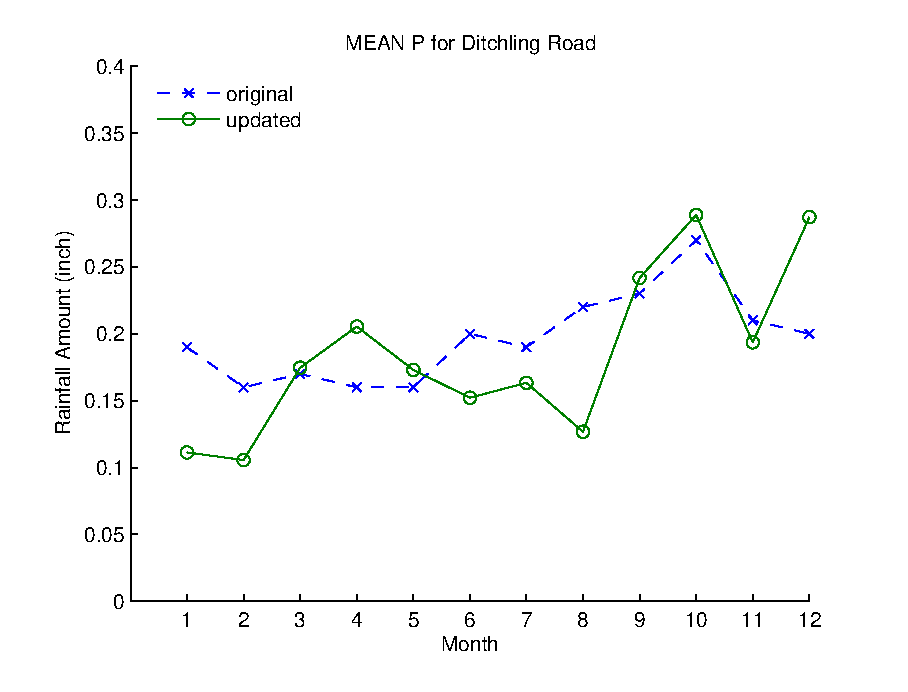
\includegraphics[width=0.60\textwidth]{mean_p_cligen}
% \caption[Mean daily precipitation depth]{Mean daily precipitation depth
%(inch)}
% \label{fig:mean_p_cligen}
%\end{figure}
%
%peak amount in autumn
%
%\begin{table}[htbp]
% \centering
% \caption[Original and Updated MX~.5P for Ditchling Road]{Original and
%Updated MX~.5P for Ditchling Road (in/hr)}
% \label{tab:UpdatedMX5PForDitchlingRoad}
%   \footnotesize
%   \begin{tabular}{lrrrrrrrrrrrr}
%   \toprule
%    & Jan & Feb & Mar & Apr & May & Jun & Jul & Aug & Sep & Oct &
%Nov & Dec\\
%   \cmidrule{2-13}
%   Original & 0.63 & 0.59 & 0.55 & 0.55 & 0.55 & 0.55 & 0.55 & 0.67
%& 0.79 & 0.93 & 0.87 & 0.75\\
%   Updated & 0.27 & 0.18 & 0.23 & 0.23 & 0.27 & 0.33 & 0.42 & 0.58
%& 0.43 & 0.45 & 0.34 & 0.30\\
%   \bottomrule
%   \end{tabular}
%\end{table}
%
%\begin{figure}[htbp]
% \centering
%   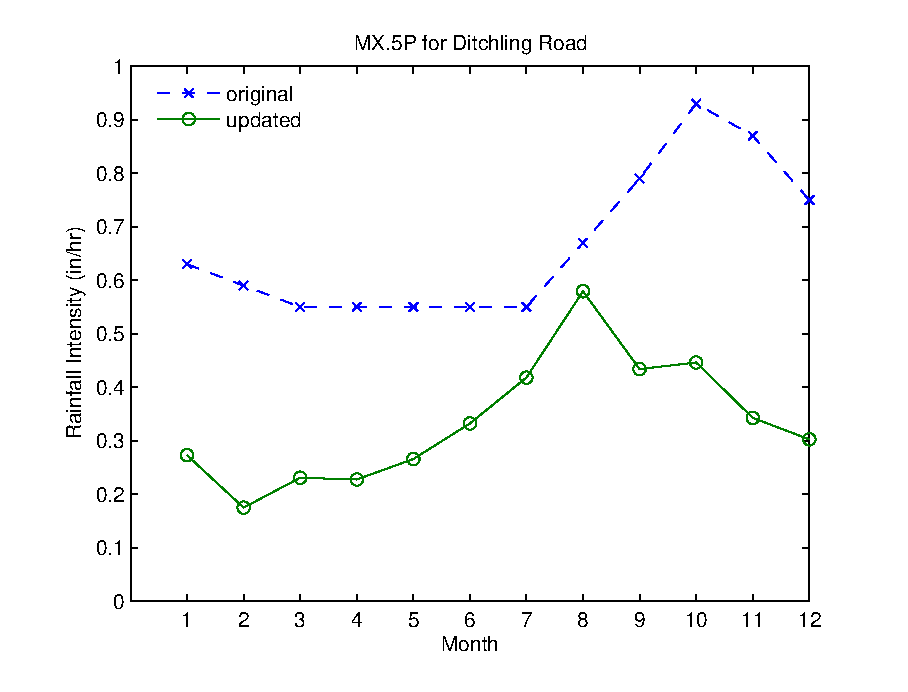
\includegraphics[width=0.70\textwidth]{mx5p_cligen}
% \caption[Mean max. daily 30-minute rainfall intensity]{Mean max. daily
%30-minute rainfall intensity (in/hr). High intensity event in summer}
% \label{fig:mx5p_cligen}
%\end{figure}
%Complete input files for both sites are shown in Appendix
%\ref{sec:CLIGENInputData}.
%
%\subsection{EUROSEM}
%\label{sec:EUROSEM}
%
%EUROSEM input settings and assumptions.
%
%\subsection{RillGrow}
%\label{sec:ModelConfigurationRillGrow}
%
%RillGrow input settings and assumptions.

\section{A Brief Overview of Research Method}
\label{sec:OverviewOfResearchMethods}

This research aims to discover how rainfall intensity changes will affect the
soil erosion rate in the future, using soil erosion models. The research method
involves data acquisition, such as observed rainfall properties and soil
properties, configuring erosion models, and sensitivity tests of erosion models.
The simulation carried out for the sensitivity test mainly employs a univariate
method.

% As this study mainly aims to investigate soil erosion changes as a response
%to future rainfall intensity changes, and future rainfall intensity changes are
%still poorly known, it is not the main focus of this study to actually attempt
%to predict future soil erosion rates. Instead, this study aims to investigate
%the way in which rainfall intensity changes can affect soil erosion rates.
%Greater knowledge here will, once future changes in rainfall intensity become
%better known, improve our ability to estimate future rates of erosion. Thus, in
%general, a ``sensitivity analysis'' approach is followed. ``Known'' rather than
%``realistic'' changes in intensity are used in this thesis.

%The thesis consists of 11 chapters in total. These chapters are divided into
%five parts: Introduction, Observed Precipitation of the Research Site, Rainfall
%Intensity Changes and Soil Erosion, Implications of Climate Change on Future
%Soil Erosion, and Conclusion.
Three soil erosion models, WEPP (Water Erosion Prediction Project), EUROSEM
(EURopean Soil Erosion Model), and RillGrow were used to simulate runoff and
erosion rate under various rainfall intensity conditions. Effects of temporal
resolution of rainfall data on runoff and soil loss generations are investigated
to identify requirements of rainfall intensity information for erosion
simulations. Two extreme rainfall events; one with highest rainfall intensity
and the other with highest rainfall amount, were selected from the
tipping-bucket rainfall data. Tipping-bucket data for the events are then
aggregated into a range of different temporal ``scales". This is done by the
discretization of tipping-bucket data into rainfall data that have a range of
time-steps (i.e. 1, 5, 15, 30 and 60min).
Runoff and soil loss rates were simulated using three models with these rainfall
input data. An additional rainfall event, which has both wet and dry phases
during the storm period, was selected. Two rainfall input data were prepared
from this event data; one without any alteration and the other that is
aggregated into a continuous storm by removing dry phases during the storm.
Runoff and soil loss rates were simulated using three models with these two
additional rainfall inputs. This was done to investigate effects of the dry
phase within a storm on soil erosion. Impacts of various rainfall intensities
patterns on soil erosion were also studied using rainfall data from a designed
storm. Four different storms that have increasing, increasing-decreasing,
decreasing and constant rainfall intensity were prepared for erosion
simulations. Rainfall amounts for all four storms were kept the same while the
intensities vary.

To understand observed trends of rainfall intensity changes, three observed
precipitation data (i.e.\ Monthly 0.5\textdegree\ grid data, daily station data
and tipping-bucket gauge data) were acquired from the South Downs, UK. Monthly
0.5\textdegree\ grid data for 100 years were analysed, firstly, to draw outlines
of long term rainfall trends in the area. Daily precipitation data from 11
stations for the various observational periods (i.e.\ 9--93 years) in the area
were then analysed, in terms of:
\begin{itemize*}
 \item daily rainfall amount,
 \item number of raindays,
 \item simple daily intensity index,
 \item number of raindays with rainfall amount $\geq$10 mm, and
 \item number of raindays with rainfall amount $\geq$20 mm.
\end{itemize*}
This gave more detailed information about the trends of rainfall in the region
than that obtained from monthly 0.5\textdegree\ grid data. Lastly, even greater
detailed rainfall trends were studied using tipping-bucket collected rainfall
data from three stations over the period of 2--13 years. This kind of high
resolution data provides very detailed information on the patterns of the
rainfall amount and intensity.

Likely future soil erosion rates were estimated only using WEPP, as the other
two models are not designed for continuous long term simulations. A hundred
year-long weather is generated by the WEPP's climate component called CLIGEN
(CLImate GENerator) as a control climate dataset. Rainfall intensity was
then increased proportionally from the control data by changing rainfall
duration, keeping rainfall amount constant. Runoff and erosion rates were
simulated using these climate data.

\subsection{Statistical Methods for Trend Investigation}
\label{StatisticalMethodsForTrendInvestigation}

Statistical methods used in this research are briefly summarized here.

\paragraph{Simple Linear Regression}
\label{sec:SimpleLinearRegression}

%REGRESSION OR CORRELATION?
%
%Select the Pearson (parametric) correlation coefficient if you can assume
%that both X and Y are sampled from Gaussian populations. Otherwise choose
%the Spearman nonparametric correlation coefficient. Don't calculate the
%correlation coefficient (or its confidence interval) if you manipulated the
%X variable.

%Calculate linear regressions only if one of the variables (X) is likely to
%precede or cause the other variable (Y). Definitely choose linear
%regression if you manipulated the X variable. It makes a big difference
%which variable is called X and which is called Y, as linear regression
%calculations are not symmetrical with respect to X and Y. If you swap the
%two variables, you will obtain a different regression line.

Linear regression function ($y=\alpha + \beta x$) was assumed where rainfall
related indicators (Table \ref{tab:RainfallIntensityIndicators}) as dependent
variables ($y$) and time as a independent variable ($x$). The regression
coefficient ($\beta$) might be used to detect trends in time series of the
indicators. The Student's $t$-test was used to test whether the trend is
statistically significant.

%If $t$-value is greater than 1.96 ($n=\infty$), reject null hypothesis
%($\beta = 0$) with $95\%$ confidence level.
%If $n=5$, $\bar{x}\pm2.776 \frac{\sigma}{n^{1/2}}$ ; if N=10: Xavg$\pm$
%2.262 sdev/N1/2 ; if N=20: Xavg$\pm$ 2.093 sdev/N1/2 ; if N=40; Xavg$\pm$
%2.023 sdev/N1/2 ; and for ``arge'' N: Xavg$\pm$ 1.960 sdev/N1/2


\paragraph{Mann-Kendall's Test}
\label{sec:MannKendallSTest}

Mann-Kendall's test is a non-parametric test for the detection of trend in a
time series. This is primarily used because it has no linearity assumption.
Since the first proposals of the test by \citet{mann1945-245} and
\citet{kendall1975-202}, covariances between Mann-Kendall statistics were
proposed by \citet{dietz1981-169} and the test was extended in order to include
seasonality \citep{hirsch1984-727}, multiple monitoring sites
\citep{lettenmaier1988-505} and covariates representing natural fluctuations
\citep{libiseller2002-71}.

%This section should be about Kendall's rank correlation.
%look at the matlab script!

The Mann-Kendall rank correlation \citep{mann1945-245,kendall1975-202} is
sensitive to both linear and non-linear trends. This is a non-parametric method
and is based on ranking of a time series, using only the relative ordering of
ranks \citep{press1996-933}. It does not give any information about the
magnitude of the trend in the actual time series but rather gives a significance
of the trend, and information on the direction of the observed trend (i.e.\
upward, downward or unchanged).

%\begin{equation}
%\label{eq:Tau}
% T=\sum^{N}_{i=1}n_i
%\end{equation}
%where, $N$ is the total number of element in the data set (no. of years).
%$n_i$ is the number of preceding element that is larger than element $x_i$
%(i=1,2,\ldots $N$).
%When $N$ is greater than 10, the distribution function of $T$ (test
%variable) is assumed to be asymptotically Gaussian.
%
%Thus, expected value, $E(T)$ is given by:
%
%\begin{equation}
%\label{eq:ExpectedTau}
% E(T)=\mu=\frac{N(N-1)}{4}
%\end{equation}
%and, variance, $var(T)$ is given by:
%
%\begin{equation}
%\label{eq:VarianceTau}
% var(T)=\sigma^2=\frac{N(N-1)(2N+5)}{72}
%\end{equation}
%The normalised test variable, $Z(T)$, is given by:
%
%\begin{equation}
%\label{eq:NormalisedTestVariable}
% Z(T)=\frac{T-E(T)}{\sqrt{var(T)}}
%\end{equation}
%
%If $|Z(T)| > 1.96$, $H_0$ shall be rejected with $95\%$ confidence level.
%When $Z(T)$ is significant, $Z(T) > 0$ or $Z(T) < 0$ defines an ascending
%or descending trend.

\paragraph{Kolmogorov-Smirnov test}
\label{sec:KolmogorovSmirnovTest}
The two sample Kolmogorov-Smirnov test is used to determine if two distributions
differ significantly. The K-S test is a non-parametric test that tests
differences between two distributions. The K-S test has the advantage of making
no assumption about the distribution of data. Its null hypothesis is that the
two samples are distributed identically. The test is sensitive to differences in
location, dispersion and skewness of the distribution \citep{sokal1995-887}.

%\begin{verbatim}
%http://en.wikipedia.org/wiki/Kolmogorov-Smirnov_test
%\end{verbatim}
%09:06, 13 September 2006
%
%$\downarrow$ need to be reworded
%
%In statistics, the Kolmogorov-Smirnov test (often called the K-S test) is
%used to determine whether two underlying probability distributions differ,
%or whether an underlying probability distribution differs from a
%hypothesized distribution, in either case based on finite samples.
%
%The one-sample KS test compares the empirical distribution function with
%the cumulative distribution function specified by the null hypothesis. The
%main applications are testing goodness of fit with the normal and uniform
%distributions. For normality testing, minor improvements made by Lilliefors
%lead to the Lilliefors test. In general the Shapiro-Wilk test or
%Anderson-Darling test are more powerful alternatives to the Lilliefors test
%for testing normality.
%
%The two-sample KS test is one of the most useful and general nonparametric
%methods for comparing two samples, as it is sensitive to differences in
%both location and shape of the empirical cumulative distribution functions
%of the two samples.
%
%empirical distribution function Fn for n observations yi is defined as
%
%\begin{equation}
% F_n(x)={\frac{1}{n}}\sum_{i=1}^n \left\{\begin{matrix}1 & \mathrm{if}\
%y_i\leq x, \\ 0 & \mathrm{otherwise}.\end{matrix}\right.
%\end{equation}
%
%The two one-sided Kolmogorov-Smirnov test statistics are given by
%
%\begin{equation}
% D_n^{+}=\max(F_n(x)-F(x))
%\end{equation}
%\begin{equation}
%     D_n^{-}=\max(F(x)-F_n(x))
%\end{equation}
%
%where F(x) is the hypothesized distribution or another empirical
%distribution. The probability distributions of these two statistics, given
%that the null hypothesis of equality of distributions is true, does not
%depend on what the hypothesized distribution is, as long as it is
%continuous.
%
%Knuth gives a detailed description of how to analyse the significance of
%this pair of statistics [citation needed]. Many people use max(Dn+, Dn-)
%instead, but the distribution of this statistic is more difficult to deal
%with.
%
%
%When the underlying independent variable is cyclic, as with day of the year
%or day of the week, then Kuiper's test is more appropriate. Numerical
%Recipes is a good source of information on this.
%
%Furthermore, the Kolmogorov-Smirnov test is more sensitive at points near
%the median of the distribution than at its tails. The Anderson-Darling test
%provides equal sensitivity at the tails.

%******This part may need to be more descriptive
%
%The research described here involves three strategic stages:
%\begin{quote}
% \begin{enumerate}
%   \item Investigation of Rainfall Intensity
%   \item Erosion Model Evaluation
%   \item Estimation of Future Soil Erosion
% \end{enumerate}
%\end{quote}
%
%For the first stage, three temporally and spatially different datasets
%(i.e.\ monthly 0.5\textdegree\ grid data, daily station data and
%tipping-bucket gauge data) are investigated to find trends in rainfall
%intensity changes.
%In the second stage, Erosion Model Evaluation assesses soil erosion models
%(e.g.\ WEPP and EUROSEM) to find out their responses to rainfall intensity
%changes. The changes in rainfall intensity are accomplished by changing the
%original intensity proportionally. This stage provides information on
%differences between the models' responses compared to real erosion system's
%responses to changed rainfall intensity.
%At the final stage, the outcomes from the previous two stages provide
%information on future rainfall intensity, and erosion model response to
%rainfall intensity changes. This information is then used to estimate
%likely ranges of future rainfall intensity changes. In turn, future soil
%erosion rate are estimated.
%
%This research may expect following outcomes:
%\begin{quote}
% \begin{enumerate}
%   \item Improvement of our understandings of rainfall intensity
%   \item Requirement of rainfall intensity information for soil
%erosion estimation
%   \item Identification of limitations of soil erosion models for
%incorporating future rainfall intensity changes
%   \item Suggestions for soil erosion model improvements
%   \item Estimation of future soil losses induced by rainfall
%intensity changes
% \end{enumerate}
%\end{quote}

%\nolinenumbers
%\linenumbers*
%\chapter{OBSERVED RAINFALL CHARACTERISTICS OF THE STUDY AREA}
\section{Observed Rainfall Characteristics Of The Study Area}
\label{sec:RainfallCharacteristicsOfTheStudyArea}

%This chapter should really focus on comparing observed intensity trends with
%what is predicted for the future---not \emph{just} looking at trends, but
%seeing how well those trends are consistent with, or different from, GCM
%predictions for the future. You should mention that here.

\subsection{Introduction}
\label{sec:ObservedRainfallIntroduction}
%******In this chapter, why observed data were analysed is to be explained.
%Also, I need to indicate what are the possible benefits taking this route
%rather than other ways such as downscaling or perturb with GCM (or RCM)
%outputs.
As stated previously, it became apparent at the early stage of this research
that RCM rainfall data could not (and still cannot) be used directly for erosion
simulations. Although RCMs and empirically downscaled data from GCMs allow
projections to be made at a finer scale than GCMs, RCM projections still vary
greatly between models in the same way as GCMs and empirical downscaling does
not attempt to correct any biases in the data from the GCMs. Even with a finer
scale than GCMs, RCM data do not hold sufficiently detailed information of
rainfall intensity that can be used directly for erosion simulations, and were
not reliable enough for this type of approach yet---and still they are not
\citep{nearing2001-229,michael2005-155,o'neal2005-165}. That is why this part of
research was carried out.

Moreover, using outputs from a model as inputs to another model will increase
the level of uncertainty because there may be compound errors originated from
both models. For example, when RCMs generate future rainfall data, these
rainfall data are in a wrong scale, that is a larger scale than what is needed
for erosion simulations. Also, rainfall intensity data that have been obtained
from these RCM-generated rainfall data will be in a wrong scale. This scale
mis-match induces the use of downscaling to make the data usable for soil
erosion modelling. During these processes, the level of uncertainty will
increase process after process. Therefore, using observed rainfall data for
erosion simulations may be more beneficial than using RCM data. It certainly is
easier to track errors from known sources such as observed rainfall data, too.

The limitation of using observed data would be that it needs correctly scaled
data to begin with and needs reasonably long data duration to be able to pick up
seasonal variations at least, if not greater. Also, it should be remembered that
this approach is to create scenarios of future rainfall which are based on
present-day rainfall, not future rainfall. Thus, this approach assume that
future rainfall trends stay the same as present-day rainfall trends.
%Is the future rainfall intensity going to be different from the present? If so,
%how is it going to be different? Is it going to increase---or decrease?

In this chapter, three different scales of observed rainfall records were
analysed to find the rainfall intensity trend---Monthly 0.5\textdegree\ grid
rainfall, daily station rainfall and event rainfall measured by tipping-bucket
gauges. The descriptions of these data are covered in Section \ref{sec:Data}.

\subsection{Method}
\label{sec:MethodsObservedRainfallCharacteristicInvestigation}
%(***REFS NEEDED to back this up, for example, refs that used observation to
%estimate trends and method I used.) %(***NOTE TO SELF Emphasise that it has
%been done before and proven, also say about pros and cons. in discussion)
All three datasets described previously (Table
\ref{tab:PrecipitationDataUsedForCurrentRainfallTrendInvestigation}) were
analysed to find out rainfall intensity trends in the area using simple linear
regression and Mann-Kendall (M-K) rank correlation. Monthly 0.5\textdegree\ grid
rainfall data and daily station rainfall data were used without any conversion.
Event rainfall data recorded by a tipping-bucket gauge are analysed.
Tipping-bucket gauge rainfall data were aggregated into 1-min rainfall data
prior to use. Rainfall amount, duration and daily maximum 1-min peak intensity
were investigated using 1-min event rainfall data.

\citet{kundzewicz2004-7} suggested a number of tests for trend detection:
Spearman's rho, Kendall's tau/Mann-Kendall test, Seasonal Kendall test, Linear
regression and other robust regression tests.
\citet{hannaford2006-1237} also used three methods (i.e.\ M-K rank, Spearman's
rho and linear regression) to assess trends in UK runoff and low flows. They
found a good agreement between the detection rate of trends between the three
trend-testing methods.
More studies have observed a high degree of equivalence between M-K rank and
Spearman's rho tests \citep{yue2002-254} and M-K rank and linear regression
\citep{svensson2005-811}

\citet{yue2002-254} investigated the power of M-K rank and Spearman's rho. They
found that both have similar power in detecting a trend to the point of being
indistinguishable in practice. \citet{yue2002-254} said ``The power of M-K rank
test depends on the pre-assigned significance level, magnitude of trend, sample
size, and the amount of variation within a time series. That is, the bigger the
absolute magnitude of trend, the more powerful are the tests; as the sample size
increases, the tests become more powerful; and as the amount of variation
increases within a time series, the power of the tests decrease. When a trend is
present, the power is also dependent on the distribution type and skewness of
the time series.''

Thus, two trend test methods, that are linear regression and M-K rank, are used
in this section.

The trends in daily rainfall characteristics were investigated. Rainfall related
indicators were calculated to determine rainfall characteristics (Table
\ref{tab:RainfallIntensityIndicators}). Daily rainfall intensity is obtained by
dividing the monthly rainfall amount by the number of raindays.

\begin{table}[htbp]
  \figureversion{tabular}
  \centering
  \caption{Rainfall intensity indicators}
  \label{tab:RainfallIntensityIndicators}
  \footnotesize
    \begin{tabular}{l p{95mm} l}
    \toprule
    \textbf{Indicator} & \textbf{Definition} & \textbf{Unit}\\
    \midrule
    RR & Precipitation sum & mm\\
    RR1 & Number of wet days (RR $\geq$ 1 mm/day) & days\\
    SDII & Simple daily intensity index: \[\frac{\textrm{total
rainfall amount for wet days (RR $\geq$ 1 mm/day)}}{\textrm{number of wet days}}
\] & mm/day\\
    %\addlinespace[-2.5mm]
    R10mm & No. of days with precipitation $\geq$ 10 mm/day & days\\
    R20mm & No. of days with precipitation $\geq$ 20 mm/day & days\\
    R10p$^\dagger$ & Ratio of days with precipitation $\geq$ 10
mm/day ((R10/RR1)$\times100$) & \%\\
    R20p$^\dagger$ & Ratio of days with precipitation $\geq$ 20
mm/day ((R20/RR1)$\times100$) & \%\\
    \bottomrule
%   \addlinespace[1mm]
    \multicolumn{3}{p{12cm}}{\footnotesize $^\dagger$\ Additional
indicators, which are not listed in the European Climate Assessment \& Dataset
project (ECA\&D) website. Complete list of indicators and their definitions are
available at http://eca.knmi.nl/indicesextremes/indicesdictionary.php}
    \end{tabular}
\end{table}

Any year with partial records were discarded to minimize the effects from
missing data (Table \ref{tab:DailyRainfallStationsAndRecordDetails}).
The records of the last year of each station were also discarded as they are
incomplete. For example, daily rainfall data from Falmer Farm (FF) were
considered only for 1904--1996 discarding the records for 1997 and 1999 with
missing data. Three more years (1998, 2000 and 2001) were discarded from all the
stations because of the discontinuity resulted in by removing missing data
periods. Also, there was a problem with 2000 rainfall because they were recorded
as weekly total rather than daily total.

\begin{table}[htbp]
  \figureversion{tabular}
  \centering
  \caption{Daily Rainfall Stations and Record Details }
  \label{tab:DailyRainfallStationsAndRecordDetails}
  \small
    \begin{tabular}{llll} \toprule
    \textbf{Code} & \textbf{Station Name} & \textbf{Periods}* &
\textbf{Studied Periods}*\\
    \midrule
    DR & Ditchling Road & 1980--1989 (10) & 1980--1988 (9)\\
    SO & Southover & 1980--1998 (19) & 1980--1997 (18)\\
    PL & Plumpton & 1980--2000 (21) & 1980--1998 (19)\\
    PB & Poverty Bottom & 1980--1998 (19) & 1980--1997 (18)\\
    SDR & Seaford D. Road & 1980--2000 (21) & 1980--1999 (20)\\
    EW & Eastbourne Wilmington & 1980--2000 (21) & 1980--1999 (20)\\
    FT & Friston Tower & 1980--2000 (21) & 1980--1999 (20)\\
    LI & Litlington & 1980--2000 (21) & 1980--1999 (20)\\
    HPF & High Park Farm & 1974--2004 (31) & 1975--2003 (29)\\
    HD & Housedean & 1967--2004 (39) & 1968--2003 (37)\\
    FF & Falmer Farm & 1904--2002 (99) & 1904--1996 (93)\\
    \bottomrule
    %\addlinespace[1mm]
    \multicolumn{4}{l}{\footnotesize * (\ ): Number of years}
    \end{tabular}
\end{table}

There are some missing data periods for event data from Ditchling Road (DR) and
Southover (SO) as well. All the years with any missing data period was
discarded. Thus, only 9, 4 and 2 year-long data were used from Ditchling Road
(DR), Southover (SO) and Plumpton (PL) stations, respectively.

In this research, daily rainfall is defined as the total rainfall that fell in a
24-hour period beginning at 9:00 am, and the day is indicated by the date on
which the period begins. For example, precipitation of 5.2 mm on 29 July 2001
means that the cumulative amount of precipitation between 9:00 am, 29 July 2001
and 9:00 am, 30 July 2001 was 5.2 mm. A ``midnight to midnight'' approach is
rarely used for rainfall data records because of practical difficulties for
observation. British Summer Time (BST) is not considered here. A wet day is also
defined when the amount of daily precipitation is equal to or more than 0.2 mm.

All no-rain periods within a day were removed from 1-min event rainfall data,
and rainfall durations were calculated as effective durations. It has been
assumed that there is only one storm on a given wet day, and rainfall is
continuous during that storm. This approach was used for CLIGEN to parametrise
daily rainfall storm. Rainfall intensity was calculated by dividing rainfall
amount by the effective duration.

\subsection{Monthly Precipitation}
\label{sec:HalfDegreeGridMonthlyPrecipitationData}

Observed mean annual rainfall amount from the studied 0.5\textdegree\ grid
during 1901--2000 period is 902.6 mm.
Annual rainfall amount which is calculated from monthly grid data show no
significant trend (Figure \ref{fig:grid_annual_amount}).

\begin{figure}[htbp]
  \centering
    \includegraphics[width=0.7\textwidth]{./img/grid_annual_amount}
  \caption{Annual rainfall amount trend of monthly grid data}
  \label{fig:grid_annual_amount}
\end{figure}

There is no statistically significant trend in seasonal rainfall amounts
(Figure \ref{fig:grid_DJF_trend}).

\begin{figure}[htbp]
  \centering
    \subfloat[][DJF]{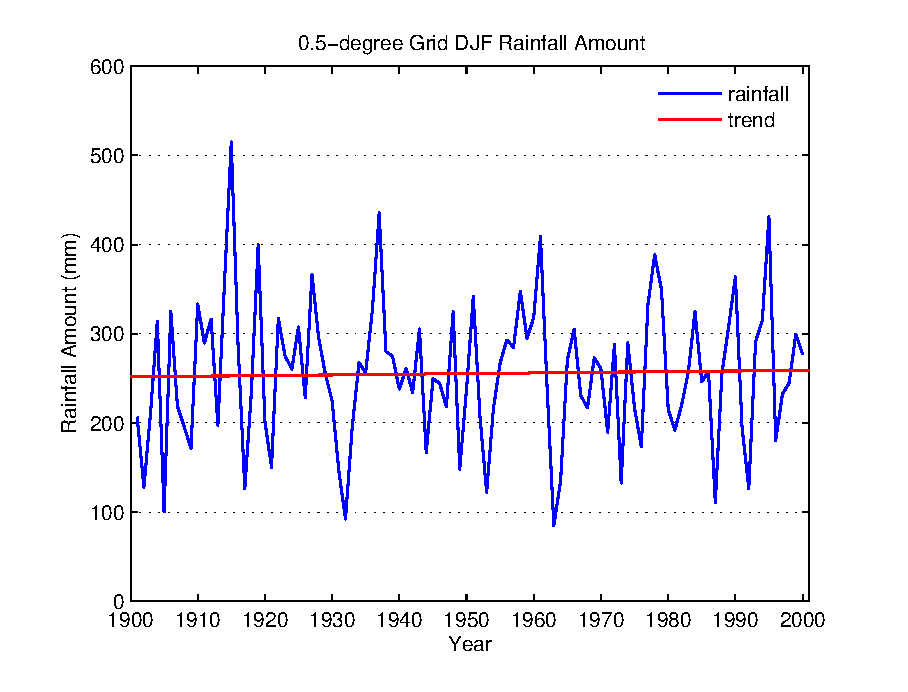
\includegraphics[width=0.5\textwidth]
{./img/grid_DJF_trend}}
    \subfloat[][MAM]{\includegraphics[width=0.5\textwidth]
{./img/grid_MAM_trend}}

    \subfloat[][JJA]{\includegraphics[width=0.5\textwidth]
{./img/grid_JJA_trend}}
    \subfloat[][SON]{\includegraphics[width=0.5\textwidth]
{./img/grid_SON_trend}}
  \caption{Seasonal rainfall amount trend of monthly 0.5\textdegree\ grid
data}

  \label{fig:grid_DJF_trend}
\end{figure}

Monthly rainfall amount pattern shows more rainfall in autumn and winter months
with a peak in November, and less rainfall in spring and summer months (Figure
\ref{fig:grid_average_monthly}). Monthly analysis of the grid data shows more
detailed monthly trend in rainfall amount. Rainfall amounts in March show a
statistically significant ($p<0.05$) decreasing trend over 1981--2000 by both
simple linear regression and Mann-Kendall's test.

\begin{figure}[htbp]
  \centering
    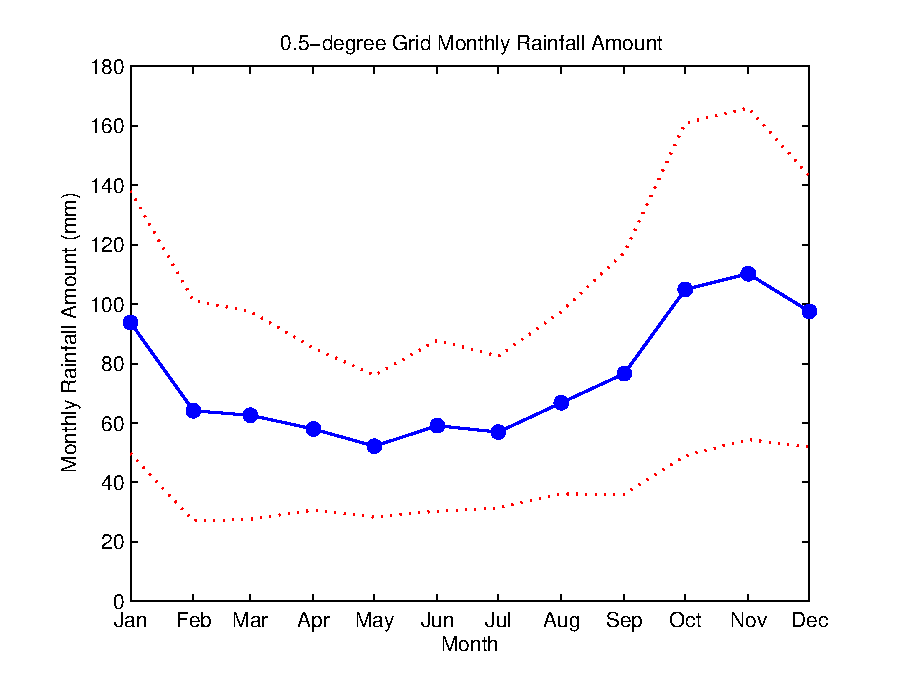
\includegraphics[width=0.7\textwidth]{./img/grid_average_monthly}
  \caption[Average monthly rainfall patterns of monthly grid data]{Average
monthly rainfall patterns of monthly grid data. Dotted lines indicate standard
deviation with 95\% confidence level.}
  \label{fig:grid_average_monthly}
\end{figure}

Rainfall amounts in July have a decreasing trend throughout the whole data
period (1901--2000) (Figure \ref{fig:grid_july_trend}).

\begin{figure}
  \centering
    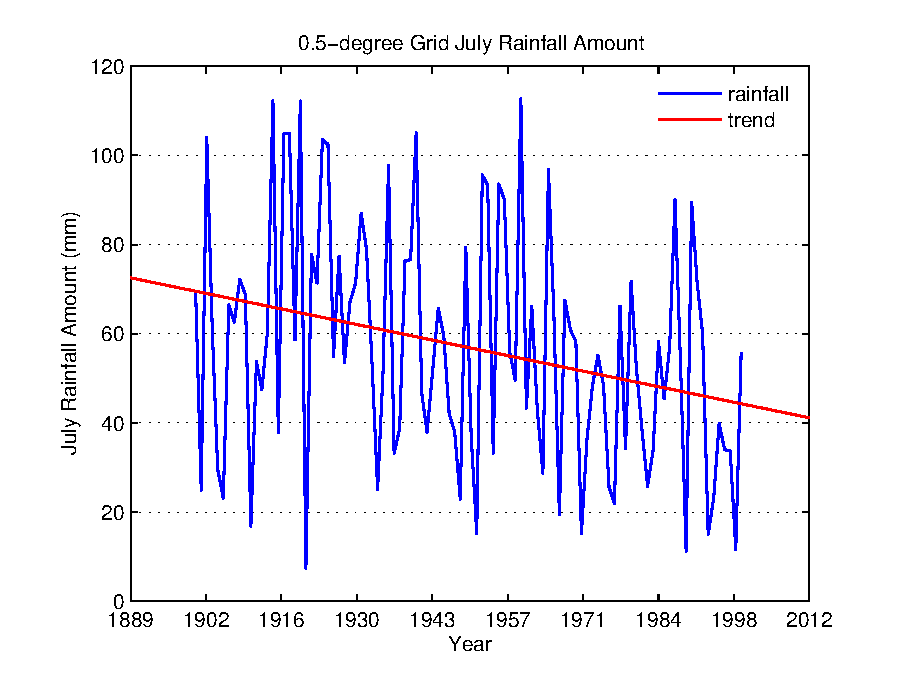
\includegraphics[width=0.7\textwidth]{./img/grid_july_trend}
  \caption{July rainfall amount trend over 1901-2000}
  \label{fig:grid_july_trend}
\end{figure}

%%%%%%%%%%%%%%%%%%%%%%%%%%%%%%%%%%%%%%%%%%%%%%%%%%%%%%%%%%
\subsection{Daily Precipitation}
\label{sec:DailyRainfallStationData}

Annual rainfall amount from Poverty Bottom (PB), Friston Tower (FT), Eastbourne
Wilmington (EW), Litlington (LI) and Seaford D. Road (SDR) stations are
significantly different from those of Plumpton (PL) or High Park Farm (HPF), for
example. This may be because of the distance from each other (see Figure
\ref{fig:DailyRainfallDataSite}) although all stations are placed in the
0.5\textdegree\ grid square.

%By stations, compare annual and monthly trend of rainfall amount and SDII.
%first of all, compare amounts for the Grid data. do this for annual and
%monthly. Are there July decrease and September increase in daily data too?
%if found and yes, it can be argued that SDII trends found in station daily
%data may be ture for the Grid Data.

\paragraph{Rainfall Amount (RR)}
\label{sec:RainfallAmountRR}

All the station show no statistically significant trend in annual rainfall
amount. This result agrees with that of monthly 0.5\textdegree\ grid rainfall
data.

For all the stations except Ditchling Road (DR), High Park Farm (HPF) and
Housedean (HD), monthly rainfall amount in March showed statistically
significant downward trends over the last two decades. The similar downward
trends are observed with rainfall amounts in July for the last decades with the
exception of DR, PB, HPF and HD stations. For longer periods, the trend of
monthly rainfall amount is inconclusive. This broadly agrees with the results
from the 0.5\textdegree\ grid data analysis. For monthly 0.5\textdegree\ grid
data, July months showed a decrease in rainfall amount.

\begin{figure}[htbp]
  \centering
  \subfloat[DR]{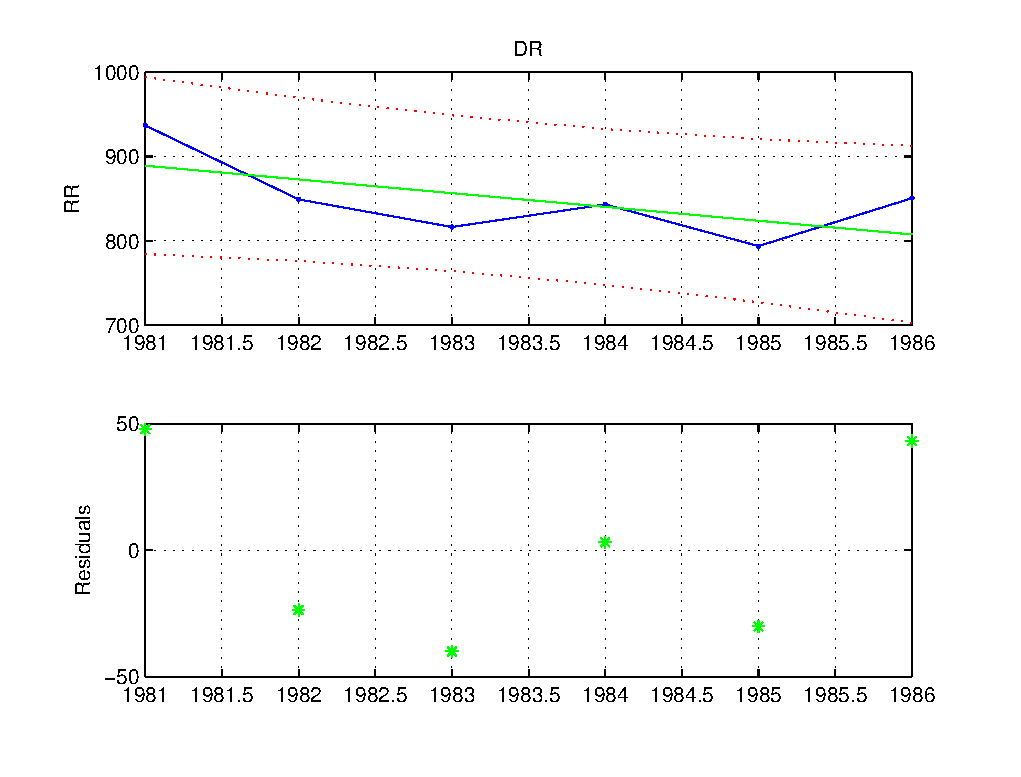
\includegraphics[width=0.33\textwidth]{./img/dr_rr}}
  \subfloat[SO]{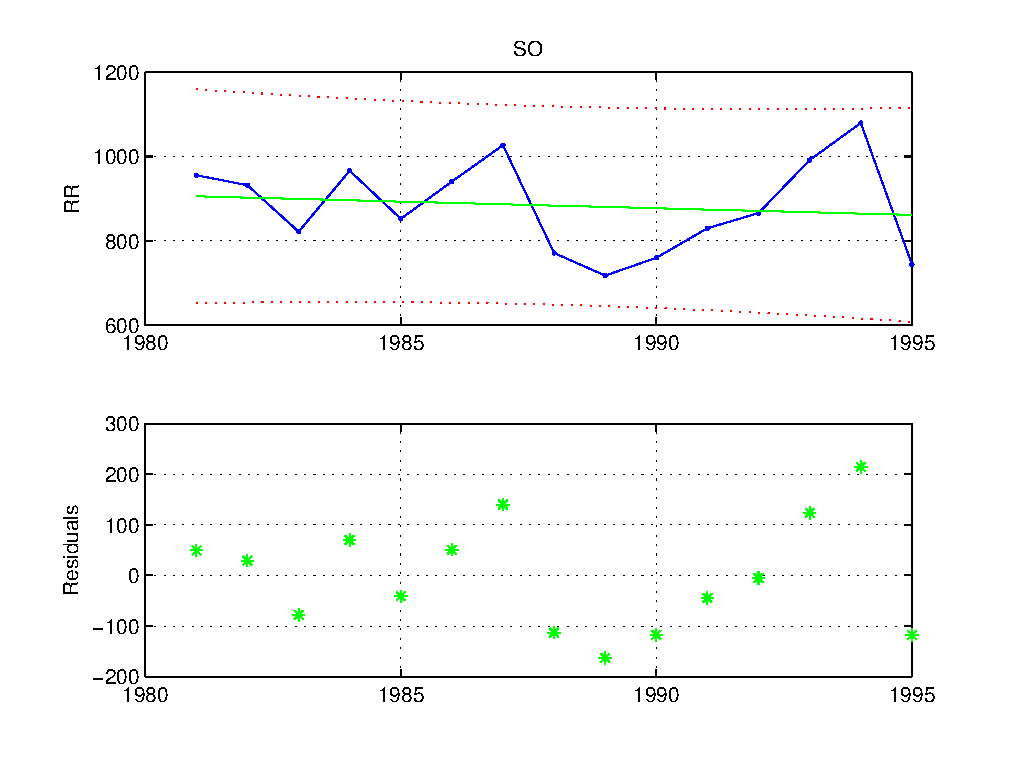
\includegraphics[width=0.33\textwidth]{./img/so_rr}}
  \subfloat[PL]{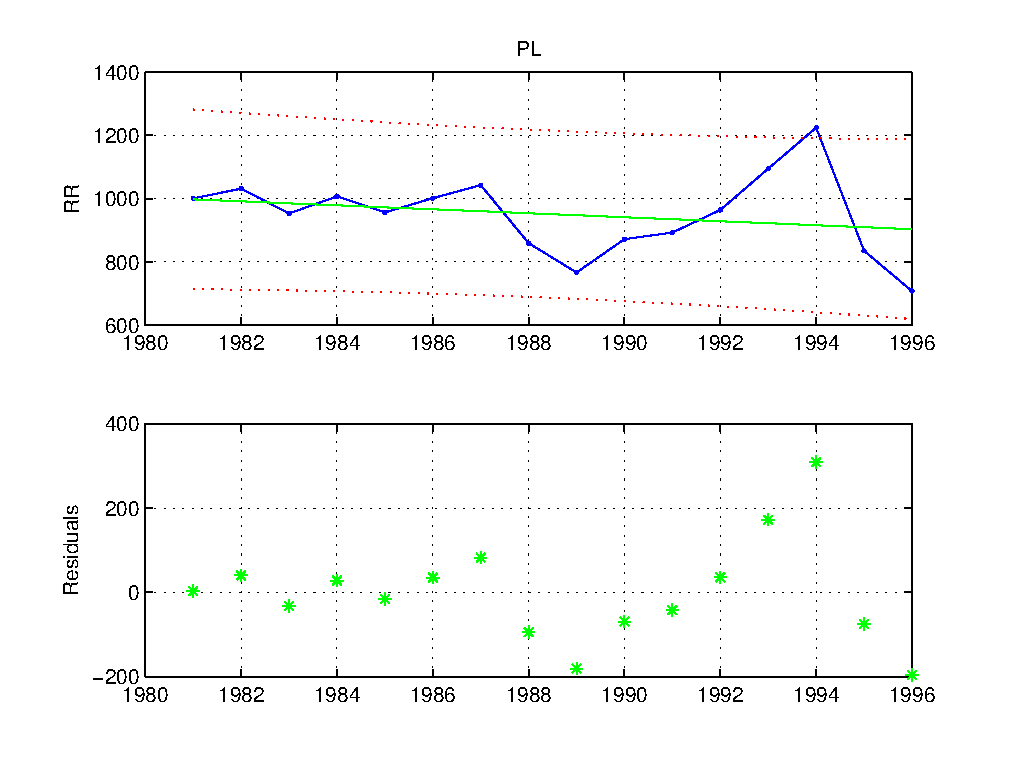
\includegraphics[width=0.33\textwidth]{./img/pl_rr}}

  \subfloat[PB]{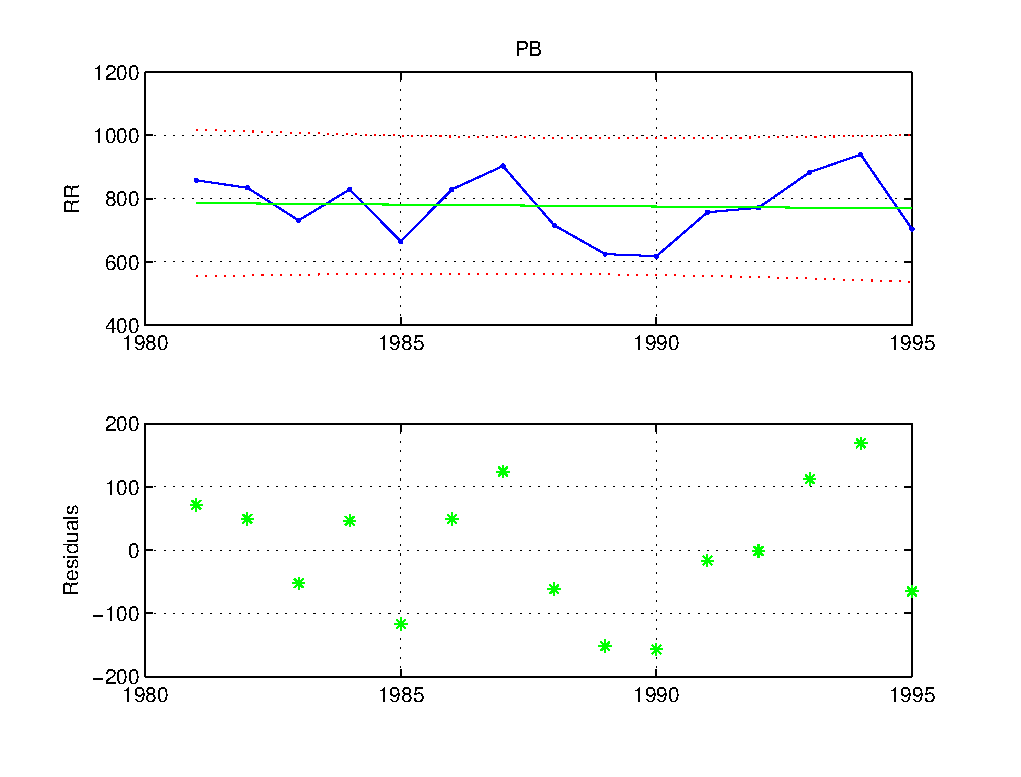
\includegraphics[width=0.33\textwidth]{./img/pb_rr}}
  \subfloat[SDR]{\includegraphics[width=0.33\textwidth]{./img/sdr_rr}}
  \subfloat[EW]{\includegraphics[width=0.33\textwidth]{./img/ew_rr}}

  \subfloat[FT]{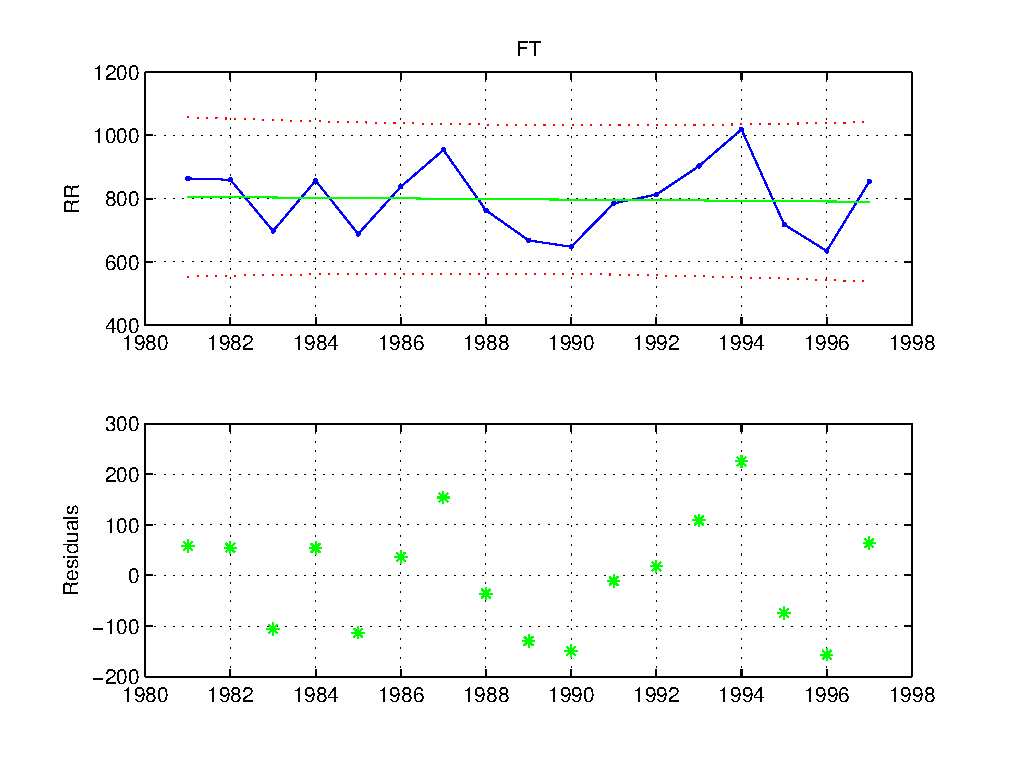
\includegraphics[width=0.33\textwidth]{./img/ft_rr}}
  \subfloat[LI]{\includegraphics[width=0.33\textwidth]{./img/li_rr}}
  \subfloat[HPF]{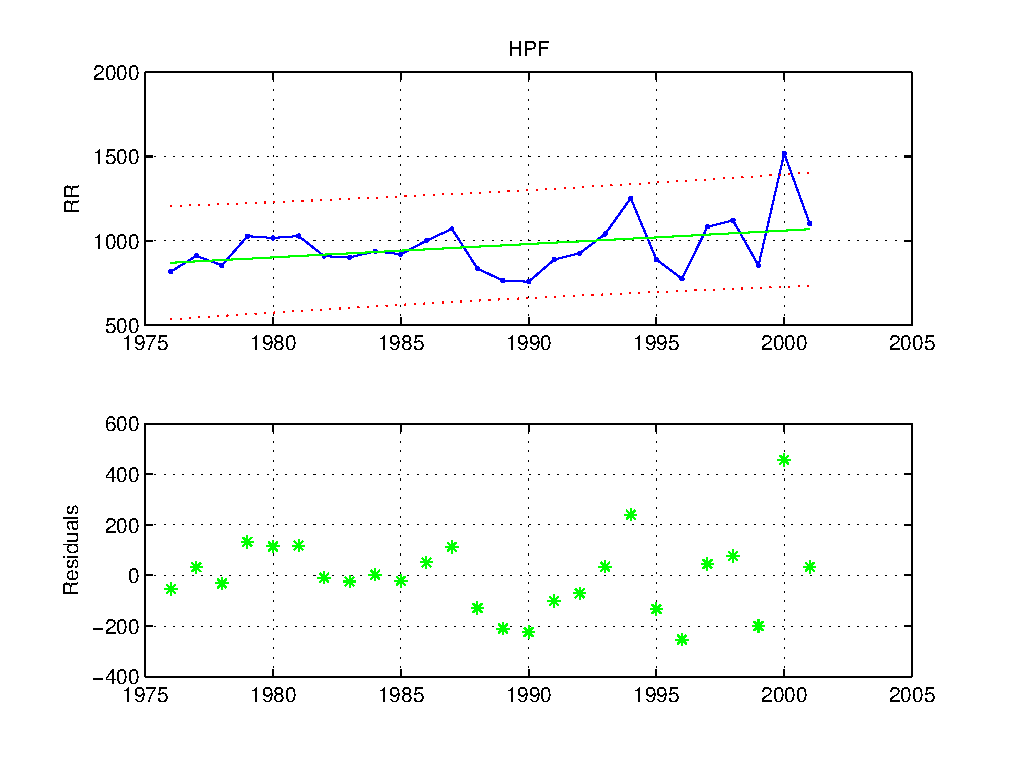
\includegraphics[width=0.33\textwidth]{./img/hpf_rr}}

  \subfloat[HD]{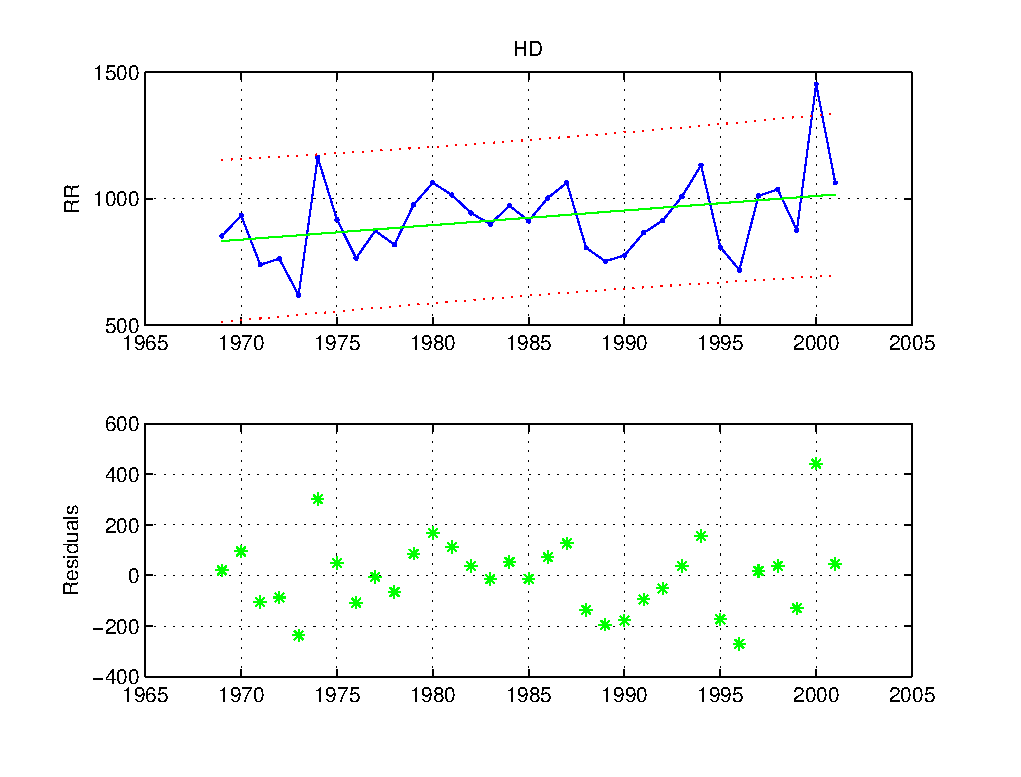
\includegraphics[width=0.33\textwidth]{./img/hd_rr}}
  \subfloat[FF]{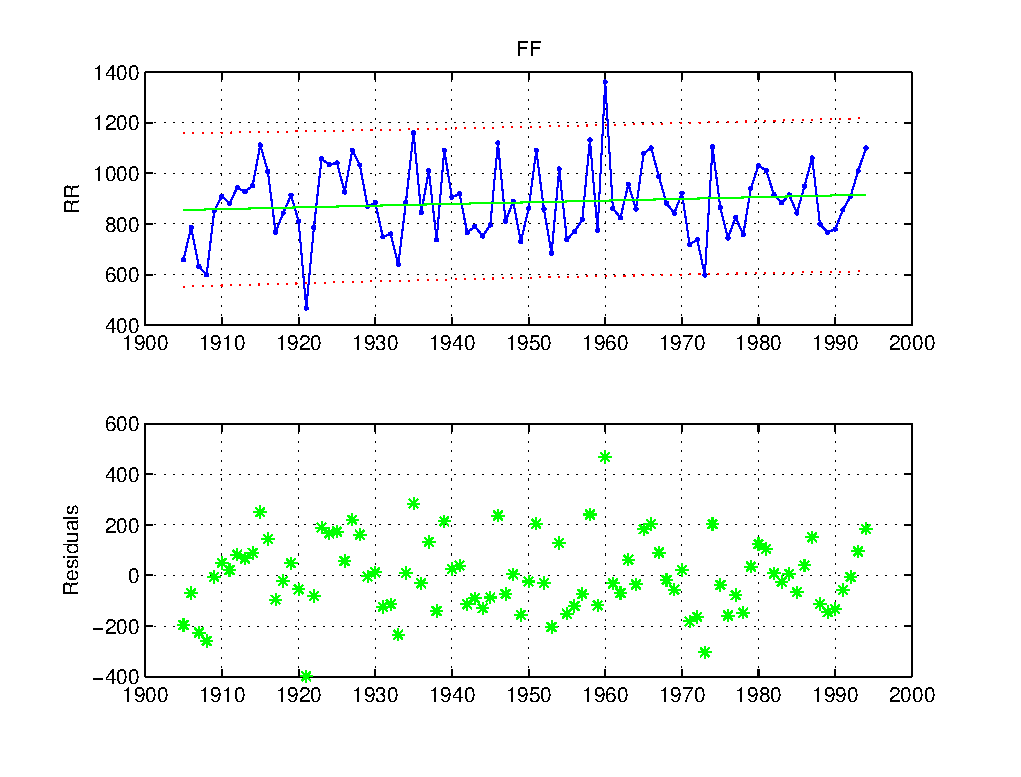
\includegraphics[width=0.33\textwidth]{./img/ff_rr}}
  \caption{Trends of annual rainfall amount (RR) at daily data stations}
  \label{fig:FF_annual_RR}
\end{figure}

\paragraph{Number of Wet Days (RR1)}
\label{sec:NumberOfRaindaysRR1}

The number of wet days per year decreased at PL and FF stations (M-K, $p<0.05$)
(Figure \ref{fig:FF_annual_RR1}). Although not all the stations showed
statistically significant annual trends, the ones with significant annual trend
in the number of wet days show downward trends in the number of wet days over
the data periods.
%A downward annual trend was also confirmed by Mann-Kendall test ($p<0.05$) for
%the same periods.

The month of March shows significant decreasing trends in the number of wet days
per month over 1980--1999. The month of July also shows decreasing trend in the
recent decade.

\begin{figure}[htbp]
  \centering
  \subfloat[DR]{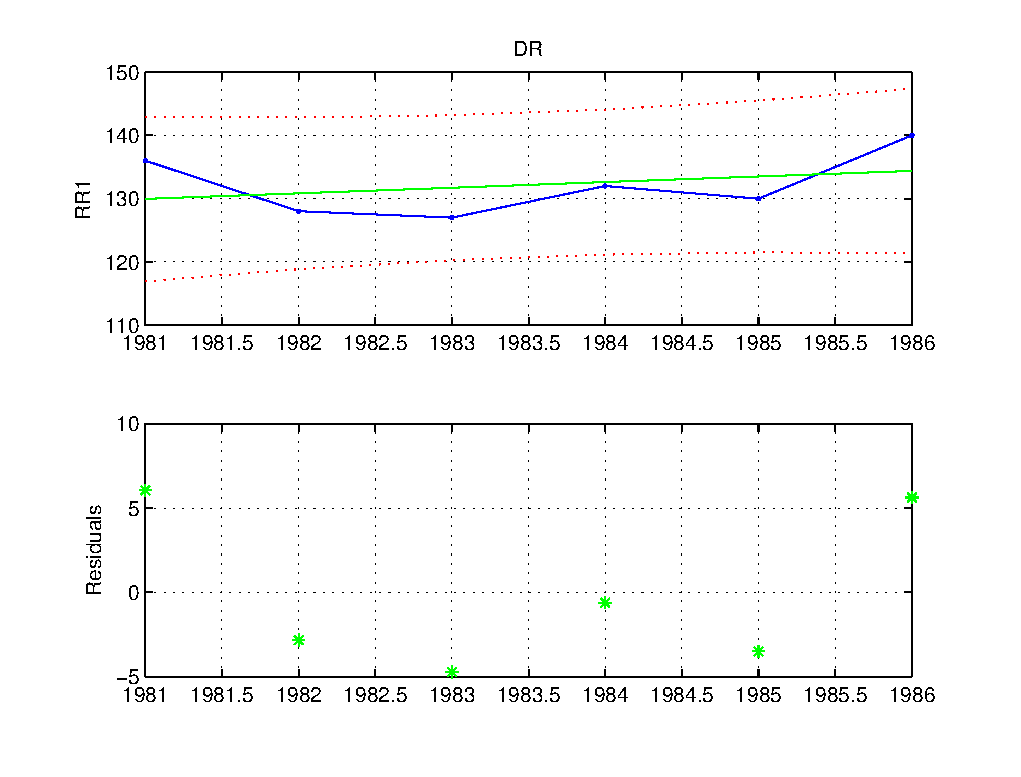
\includegraphics[width=0.33\textwidth]{./img/dr_rr1}}
  \subfloat[SO]{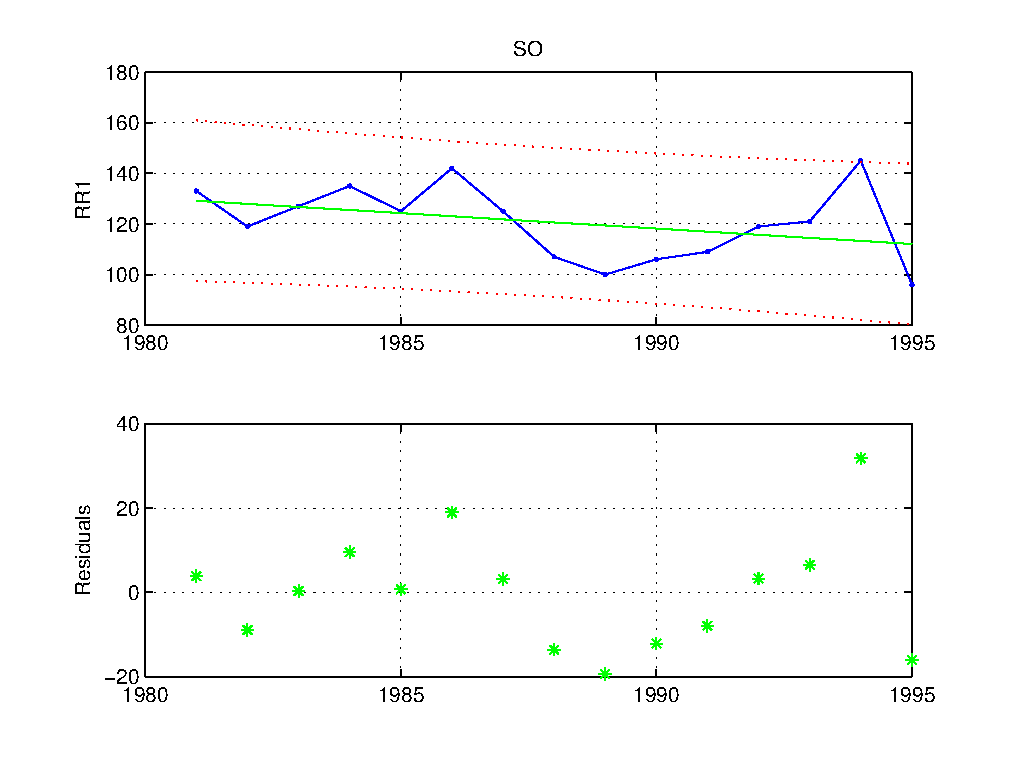
\includegraphics[width=0.33\textwidth]{./img/so_rr1}}
  \subfloat[PL]{\includegraphics[width=0.33\textwidth]{./img/pl_rr1}}

  \subfloat[PB]{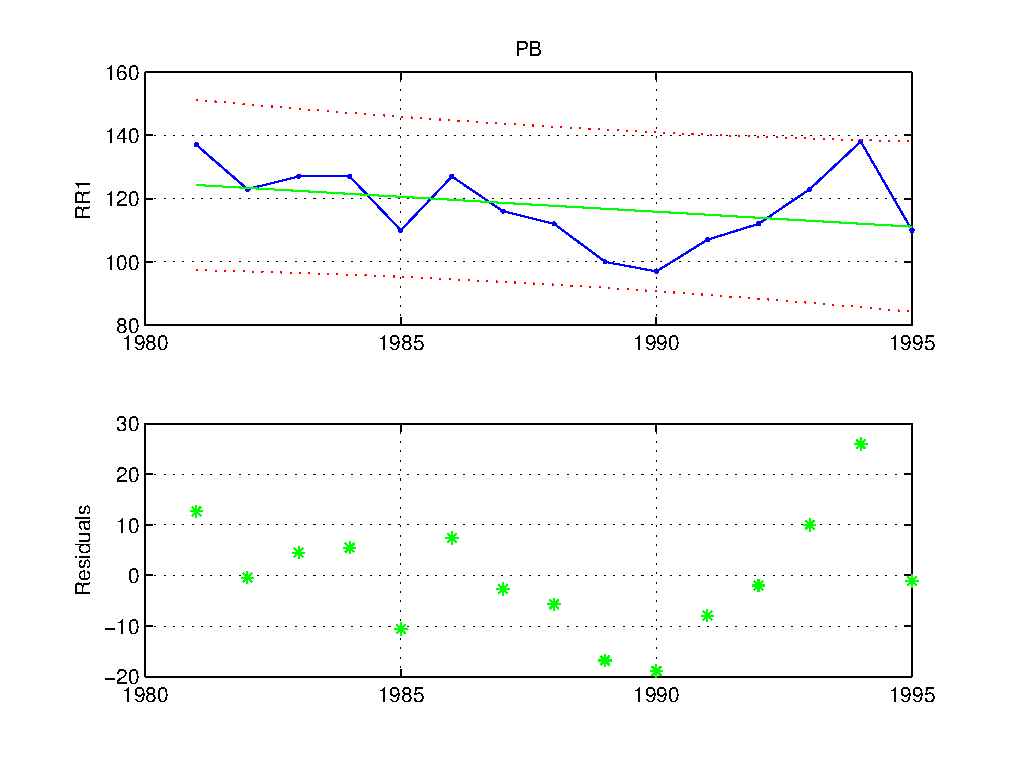
\includegraphics[width=0.33\textwidth]{./img/pb_rr1}}
  \subfloat[SDR]{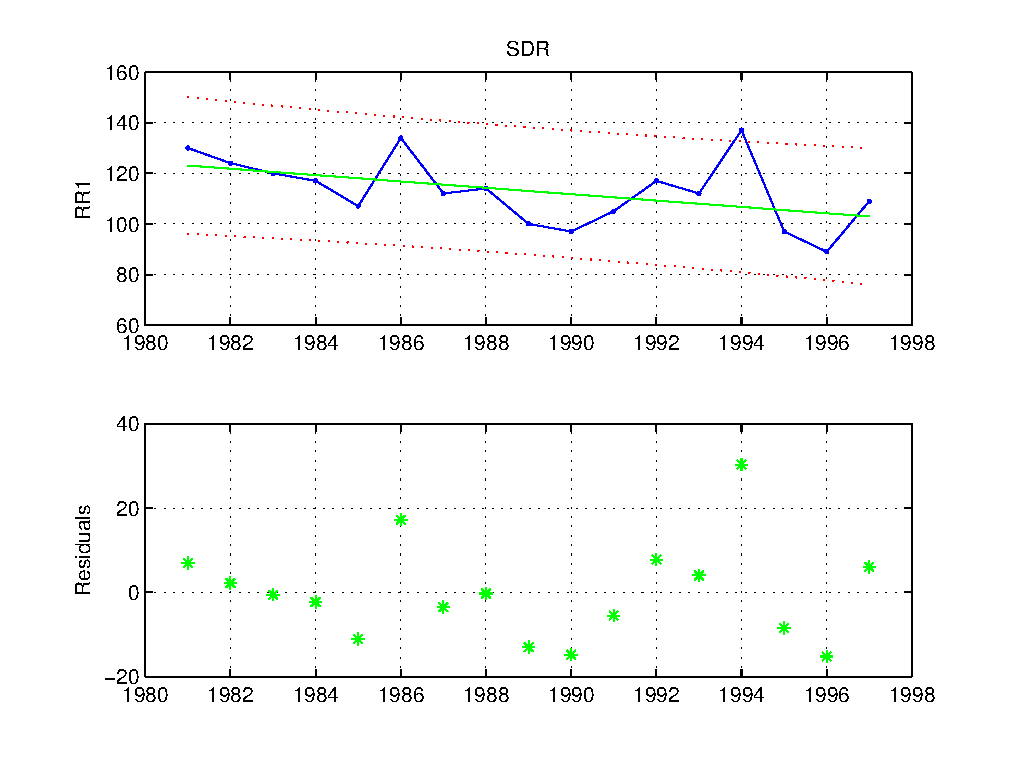
\includegraphics[width=0.33\textwidth]{./img/sdr_rr1}}
  \subfloat[EW]{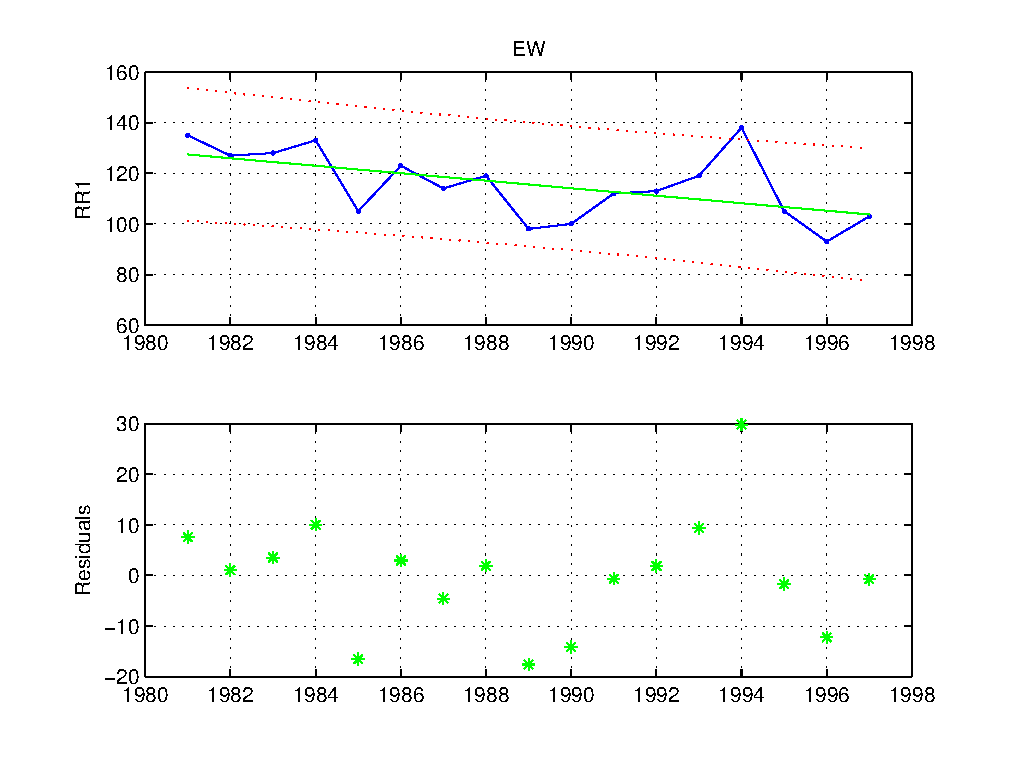
\includegraphics[width=0.33\textwidth]{./img/ew_rr1}}

  \subfloat[FT]{\includegraphics[width=0.33\textwidth]{./img/ft_rr1}}
  \subfloat[LI]{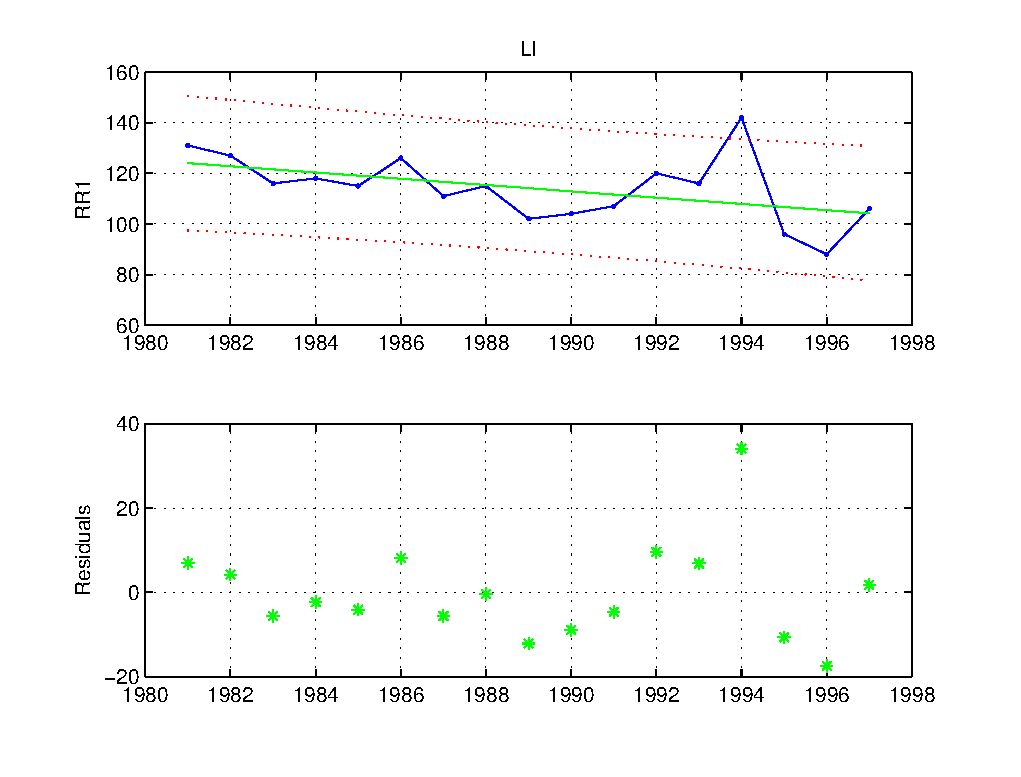
\includegraphics[width=0.33\textwidth]{./img/li_rr1}}
  \subfloat[HPF]{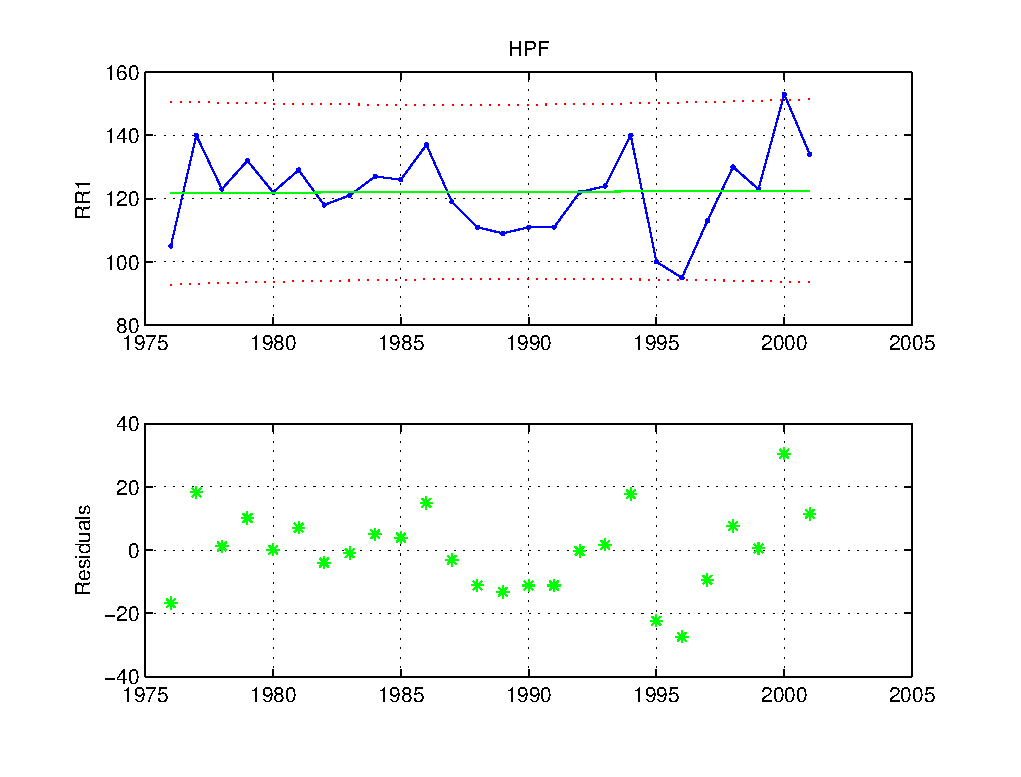
\includegraphics[width=0.33\textwidth]{./img/hpf_rr1}}

  \subfloat[HD]{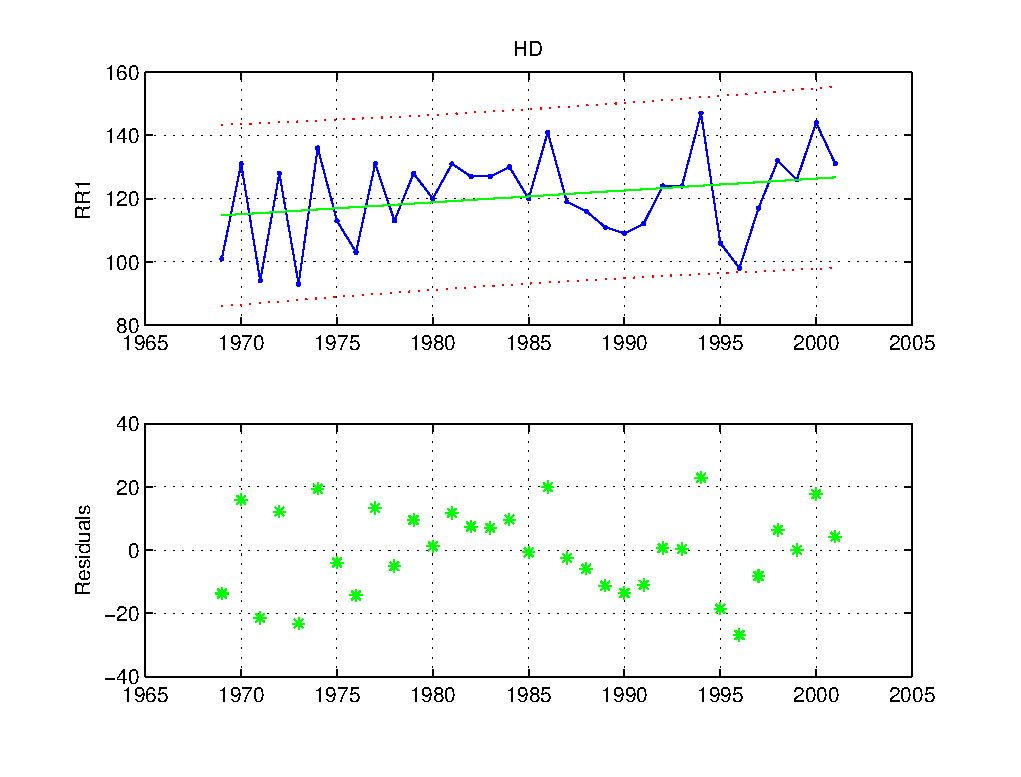
\includegraphics[width=0.33\textwidth]{./img/hd_rr1}}
  \subfloat[FF]{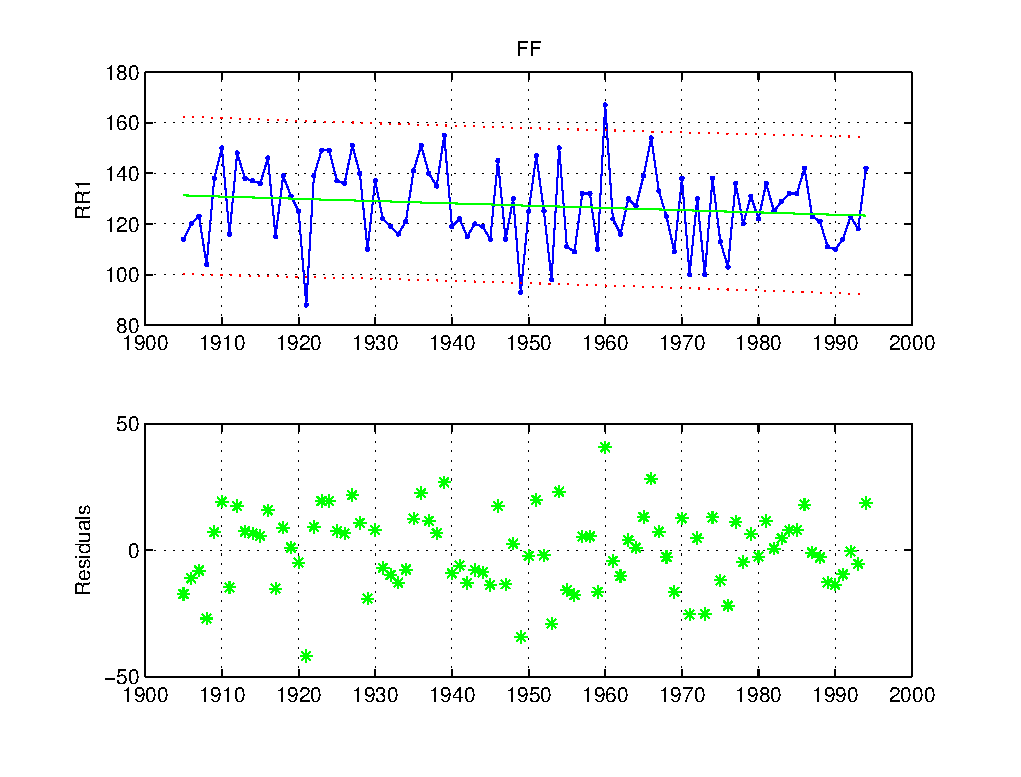
\includegraphics[width=0.33\textwidth]{./img/ff_rr1}}
  \caption{Trends of number of wetdays (RR1) at daily data stations}
  \label{fig:FF_annual_RR1}
\end{figure}

\paragraph{Simple Daily Intensity Index (SDII)}
\label{sec:SimpleDailyIntensityIndex}
As expected, PL \& FF again showed a significant annual trend in SDII. The rest
of the stations showed no significant results. FF station showed upward annual
trends in SDII throughout the data periods (Figure \ref{fig:FF_annual_SDII}).
All the cases with significant trends exhibited increasing trend of annual
SDII.

\begin{figure}[htbp]
  \centering
  \subfloat[DR]{\includegraphics[width=0.33\textwidth]{./img/dr_sdii}}
  \subfloat[SO]{\includegraphics[width=0.33\textwidth]{./img/so_sdii}}
  \subfloat[PL]{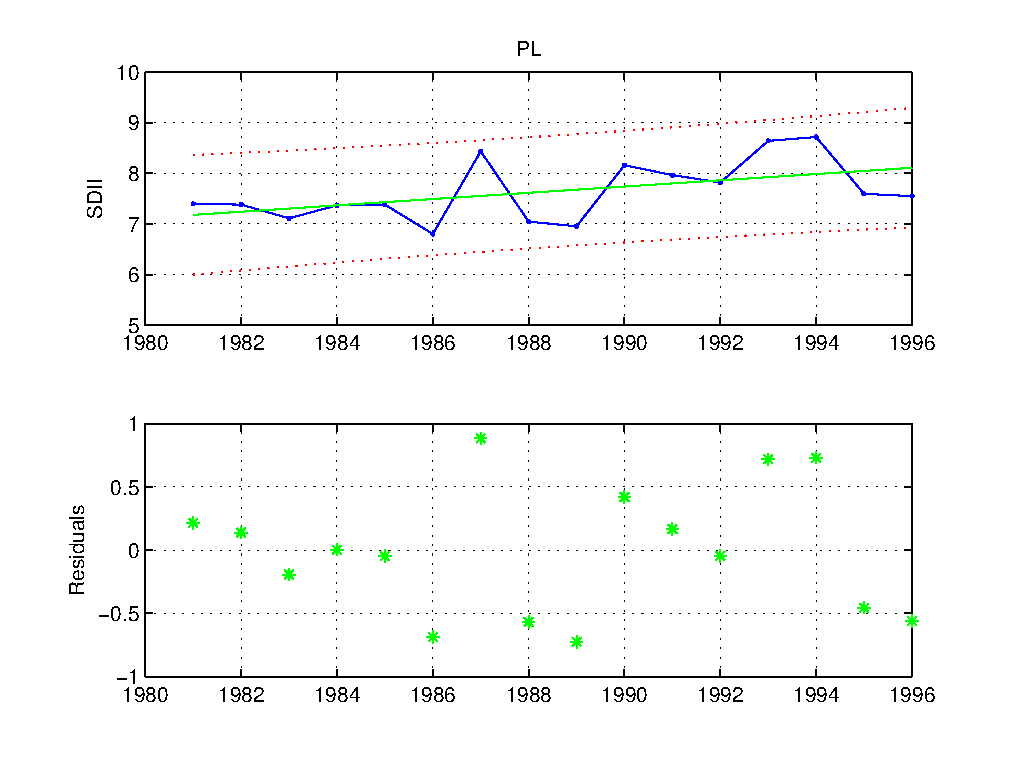
\includegraphics[width=0.33\textwidth]{./img/pl_sdii}}

  \subfloat[PB]{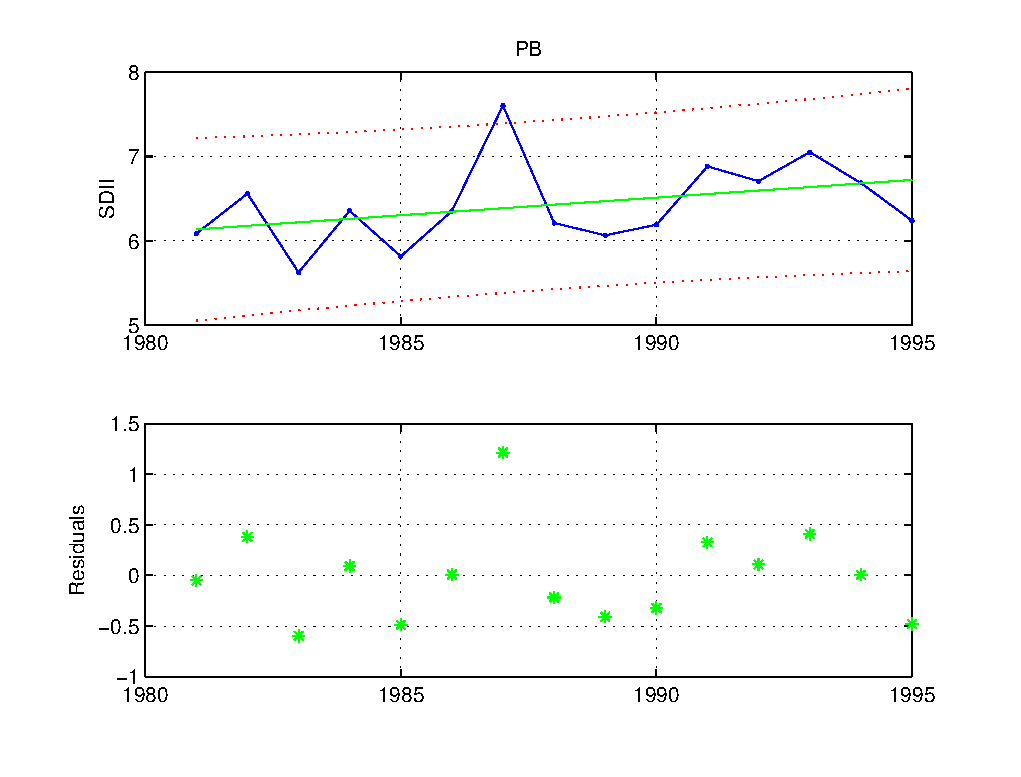
\includegraphics[width=0.33\textwidth]{./img/pb_sdii}}
  \subfloat[SDR]{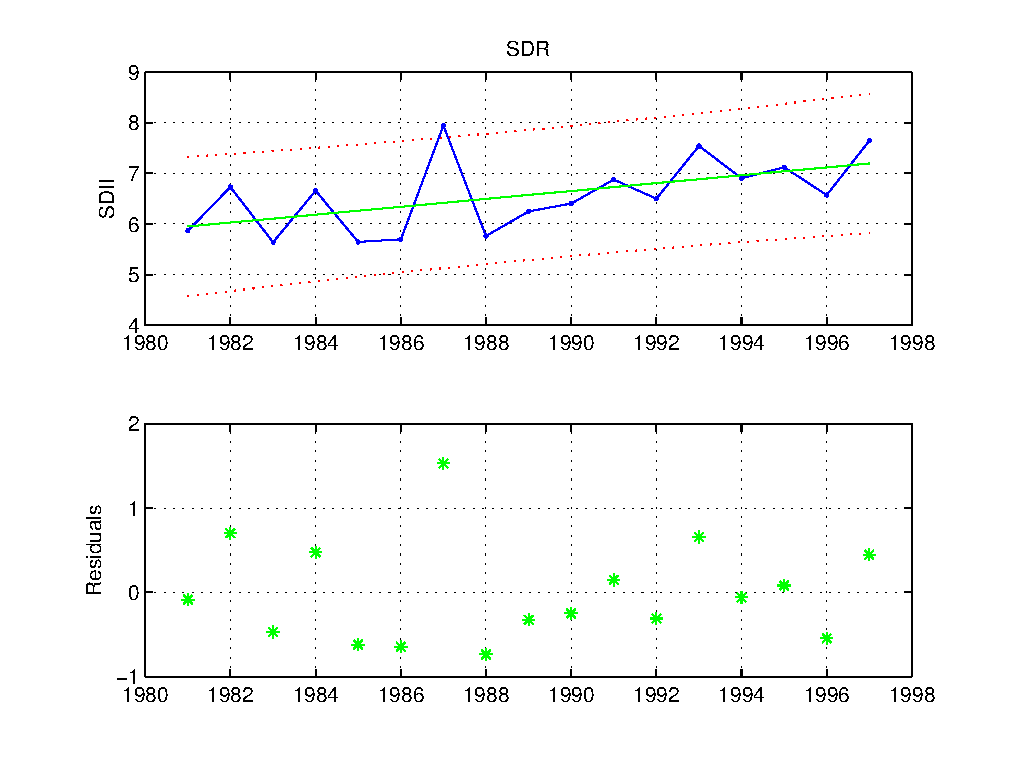
\includegraphics[width=0.33\textwidth]{./img/sdr_sdii}}
  \subfloat[EW]{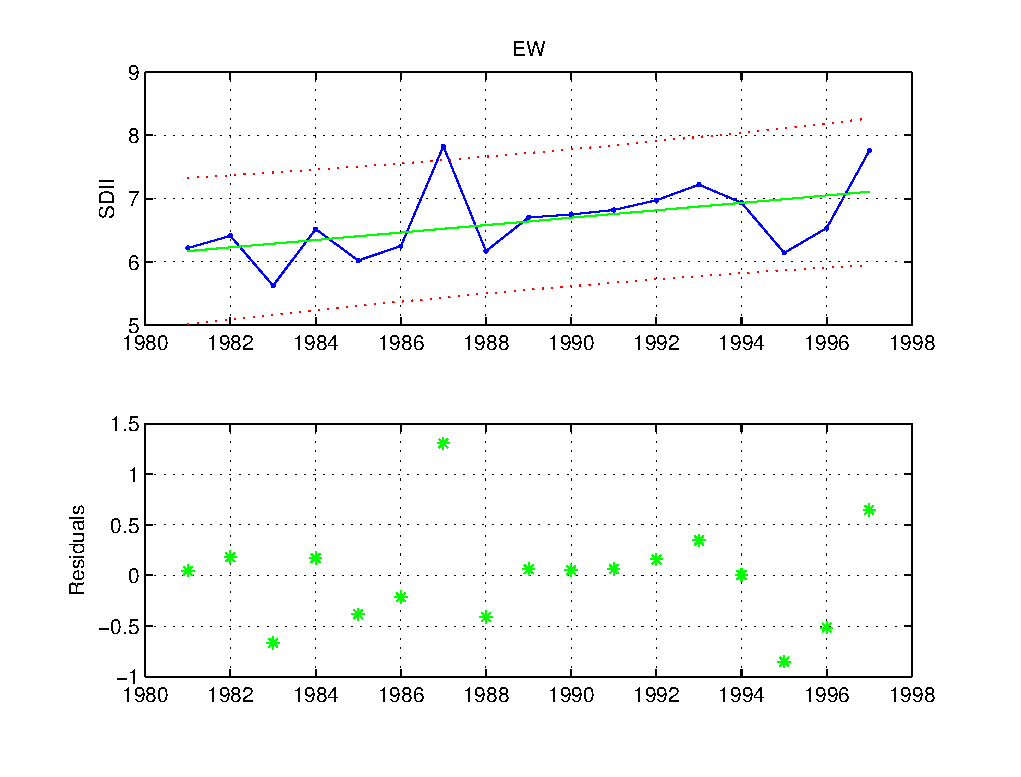
\includegraphics[width=0.33\textwidth]{./img/ew_sdii}}

  \subfloat[FT]{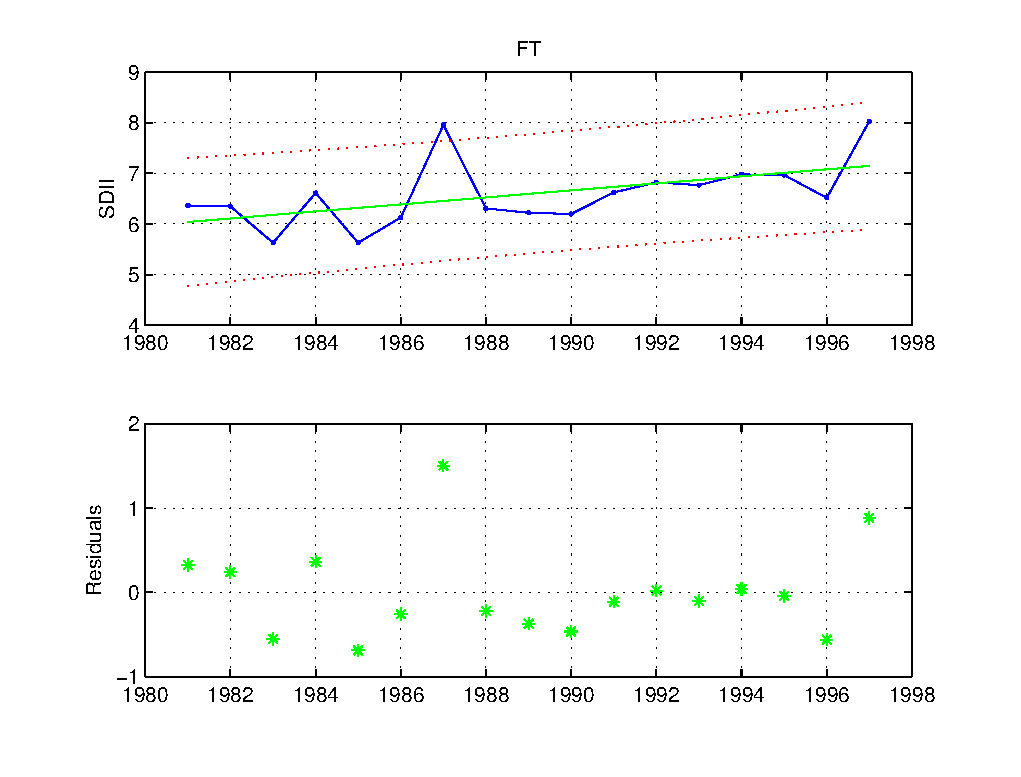
\includegraphics[width=0.33\textwidth]{./img/ft_sdii}}
  \subfloat[LI]{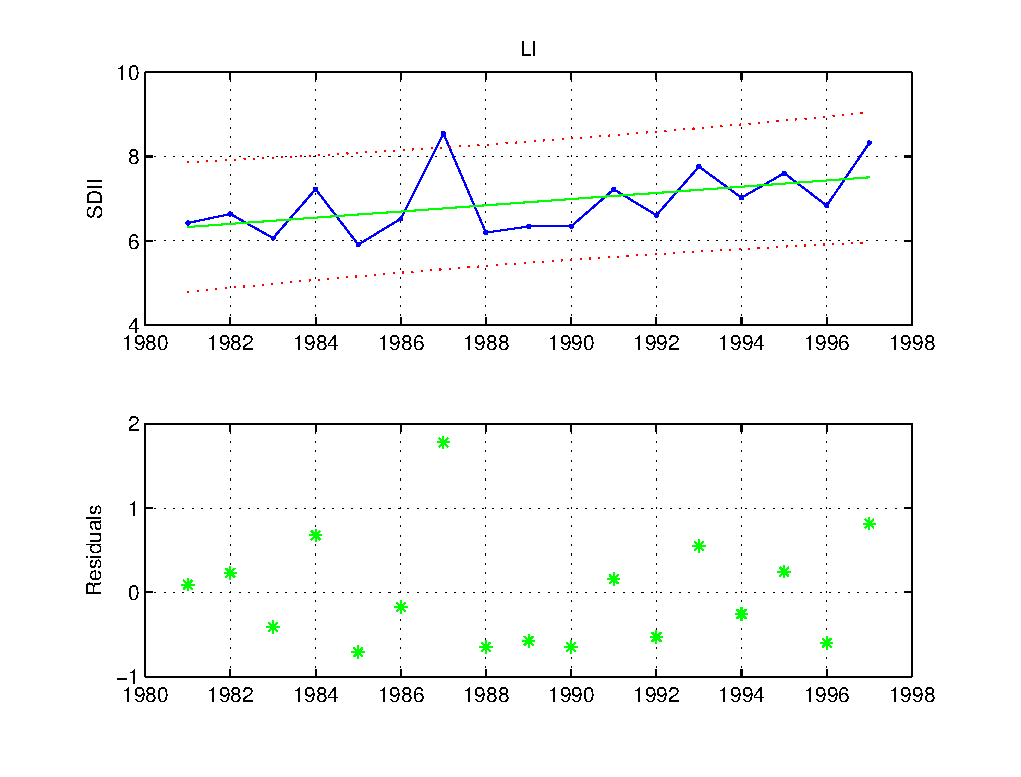
\includegraphics[width=0.33\textwidth]{./img/li_sdii}}
  \subfloat[HPF]{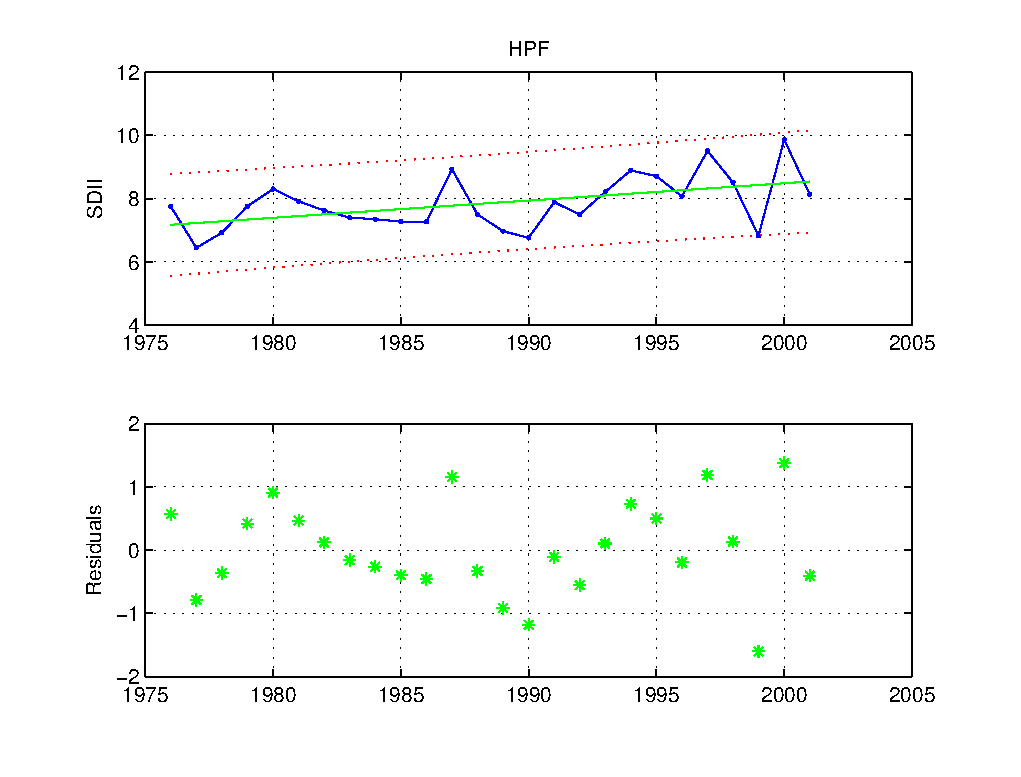
\includegraphics[width=0.33\textwidth]{./img/hpf_sdii}}

  \subfloat[HD]{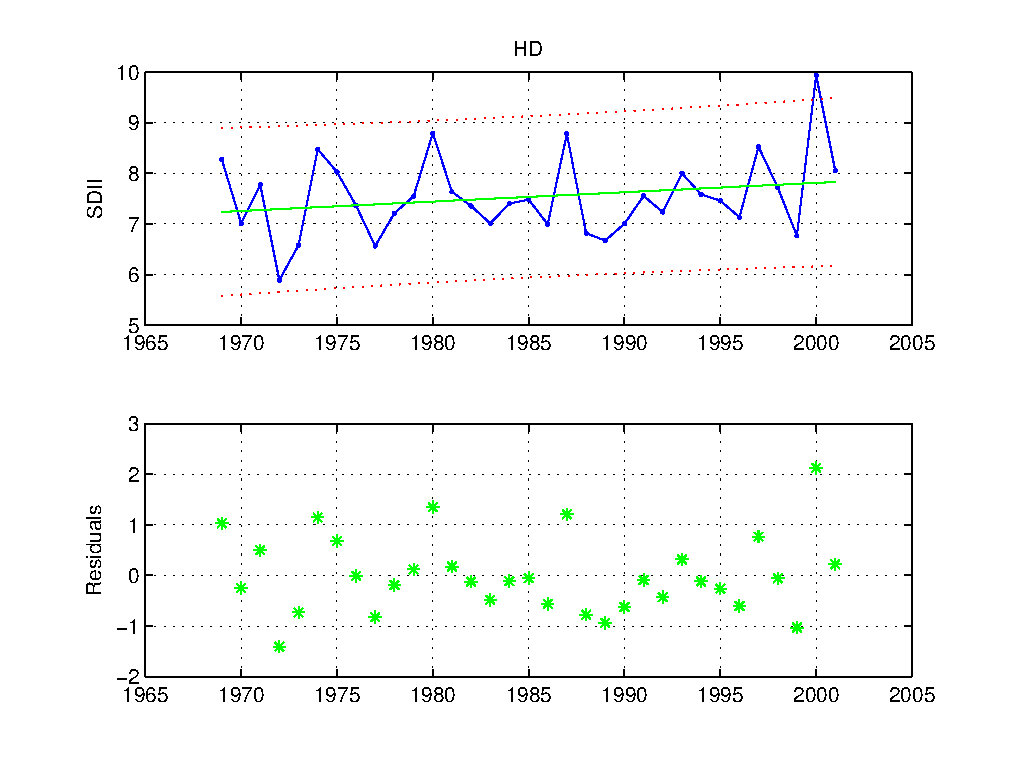
\includegraphics[width=0.33\textwidth]{./img/hd_sdii}}
  \subfloat[FF]{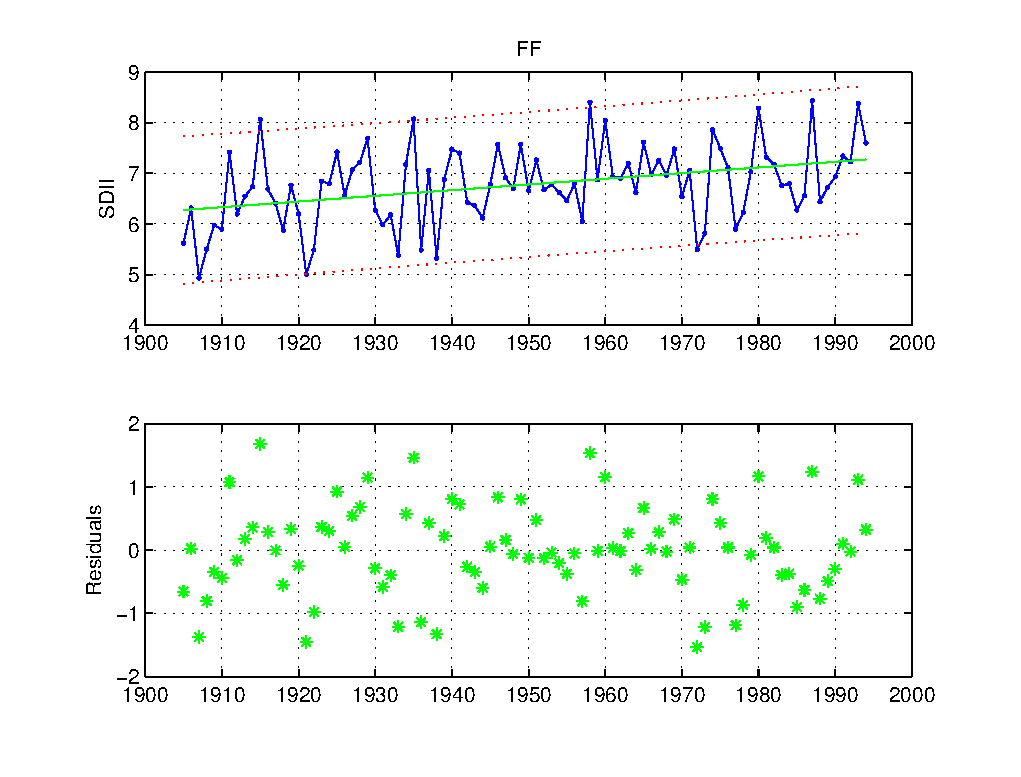
\includegraphics[width=0.33\textwidth]{./img/ff_sdii}}
  \caption{Trend of annual simple daily intensity index (SDII) at daily
data stations}
  \label{fig:FF_annual_SDII}
\end{figure}

\paragraph{Number of Days with Precipitation Amount $\geq$ 10 mm (R10mm)}
\label{sec:R10}
Annual trends of number of wet days with precipitation amount greater than 10 mm
(R10mm) from the studied stations are at variance. Only Falmer Farm Station
shows a statistically significant upwards trend for the 1971--1996 period (M-K,
$p<0.05$) (Figure \ref{fig:FF_annual_R10mm}). PL ($p < 0.05$) and FF ($p \ll
0.05$) show a statistically significant increasing trend in the annual ratio of
number of wet days with rainfall amount greater than 10 mm (Figure
\ref{fig:FF_annual_R10-b}).

\begin{figure}[htbp]
  \centering
  \subfloat[DR]{\includegraphics[width=0.33\textwidth]{./img/dr_r10mm}}
  \subfloat[SO]{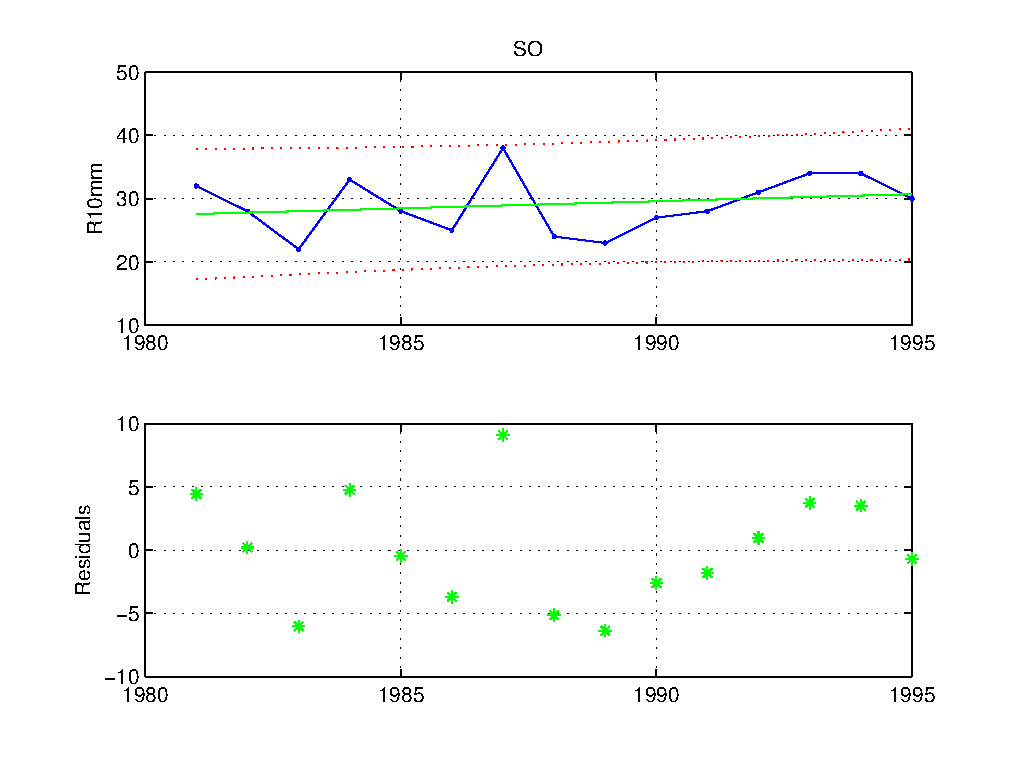
\includegraphics[width=0.33\textwidth]{./img/so_r10mm}}
  \subfloat[PL]{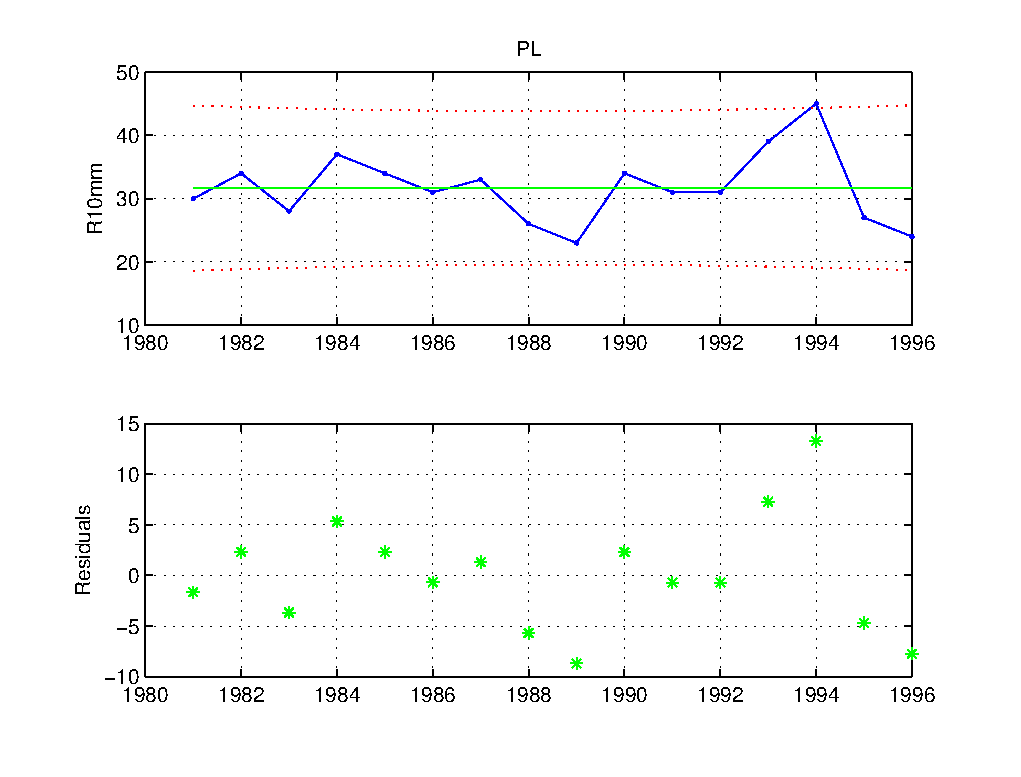
\includegraphics[width=0.33\textwidth]{./img/pl_r10mm}}

  \subfloat[PB]{\includegraphics[width=0.33\textwidth]{./img/pb_r10mm}}
  \subfloat[SDR]{\includegraphics[width=0.33\textwidth]{./img/sdr_r10mm}}
  \subfloat[EW]{\includegraphics[width=0.33\textwidth]{./img/ew_r10mm}}

  \subfloat[FT]{\includegraphics[width=0.33\textwidth]{./img/ft_r10mm}}
  \subfloat[LI]{\includegraphics[width=0.33\textwidth]{./img/li_r10mm}}
  \subfloat[HPF]{\includegraphics[width=0.33\textwidth]{./img/hpf_r10mm}}

  \subfloat[HD]{\includegraphics[width=0.33\textwidth]{./img/hd_r10mm}}
  \subfloat[FF]{\includegraphics[width=0.33\textwidth]{./img/ff_r10mm}
\label{fig:FF_annual_R10-a}}
  \caption{Annual number of wet days with rainfall amount $\geq$ 10 mm at
daily data stations}
  \label{fig:FF_annual_R10mm}
\end{figure}

\begin{figure}[htbp]
  \centering
  \subfloat[DR]{\includegraphics[width=0.33\textwidth]{./img/dr_r10p}}
  \subfloat[SO]{\includegraphics[width=0.33\textwidth]{./img/so_r10p}}
  \subfloat[PL]{\includegraphics[width=0.33\textwidth]{./img/pl_r10p}}

  \subfloat[PB]{\includegraphics[width=0.33\textwidth]{./img/pb_r10p}}
  \subfloat[SDR]{\includegraphics[width=0.33\textwidth]{./img/sdr_r10p}}
  \subfloat[EW]{\includegraphics[width=0.33\textwidth]{./img/ew_r10p}}

  \subfloat[FT]{\includegraphics[width=0.33\textwidth]{./img/ft_r10p}}
  \subfloat[LI]{\includegraphics[width=0.33\textwidth]{./img/li_r10p}}
  \subfloat[HPF]{\includegraphics[width=0.33\textwidth]{./img/hpf_r10p}}

  \subfloat[HD]{\includegraphics[width=0.33\textwidth]{./img/hd_r10p}}
  \subfloat[FF]{\includegraphics[width=0.33\textwidth]{./img/ff_r10p}
\label{fig:FF_annual_R10-b}}
  \caption{Annual \% of wet days with rainfall amount $\geq$ 10 mm at
daily data stations}
  \label{fig:FF_annual_R10p}
\end{figure}

\paragraph{Number of Days with Precipitation Amount $\geq$ 20 mm (R20mm)}
\label{sec:R20}
No station shows a significant trend in the annual number of wet days with
rainfall greater than 20 mm. A trend in the annual ratio of number of wet days
with rainfall amount over 20 mm was not detectable as well (Figure
\ref{fig:FF_annual_R20mm}).

\begin{figure}[htbp]
  \centering
  \subfloat[DR]{\includegraphics[width=0.33\textwidth]{./img/dr_r20mm}}
  \subfloat[SO]{\includegraphics[width=0.33\textwidth]{./img/so_r20mm}}
  \subfloat[PL]{\includegraphics[width=0.33\textwidth]{./img/pl_r20mm}}

  \subfloat[PB]{\includegraphics[width=0.33\textwidth]{./img/pb_r20mm}}
  \subfloat[SDR]{\includegraphics[width=0.33\textwidth]{./img/sdr_r20mm}}
  \subfloat[EW]{\includegraphics[width=0.33\textwidth]{./img/ew_r20mm}}

  \subfloat[FT]{\includegraphics[width=0.33\textwidth]{./img/ft_r20mm}}
  \subfloat[LI]{\includegraphics[width=0.33\textwidth]{./img/li_r20mm}}
  \subfloat[HPF]{\includegraphics[width=0.33\textwidth]{./img/hpf_r20mm}}

  \subfloat[HD]{\includegraphics[width=0.33\textwidth]{./img/hd_r20mm}}
  \subfloat[FF]{\includegraphics[width=0.33\textwidth]{./img/ff_r20mm}
\label{fig:FF_annual_R20-a}}
  \caption{Annual number of wet days with rainfall amount $\geq$ 20 mm at
daily data stations}
  \label{fig:FF_annual_R20mm}
\end{figure}

\begin{figure}[htbp]
  \centering
  \subfloat[DR]{\includegraphics[width=0.33\textwidth]{./img/dr_r20p}}
  \subfloat[SO]{\includegraphics[width=0.33\textwidth]{./img/so_r20p}}
  \subfloat[PL]{\includegraphics[width=0.33\textwidth]{./img/pl_r20p}}

  \subfloat[PB]{\includegraphics[width=0.33\textwidth]{./img/pb_r20p}}
  \subfloat[SDR]{\includegraphics[width=0.33\textwidth]{./img/sdr_r20p}}
  \subfloat[EW]{\includegraphics[width=0.33\textwidth]{./img/ew_r20p}}

  \subfloat[FT]{\includegraphics[width=0.33\textwidth]{./img/ft_r20p}}
  \subfloat[LI]{\includegraphics[width=0.33\textwidth]{./img/li_r20p}}
  \subfloat[HPF]{\includegraphics[width=0.33\textwidth]{./img/hpf_r20p}}

  \subfloat[HD]{\includegraphics[width=0.33\textwidth]{./img/hd_r20p}}
  \subfloat[FF]{\includegraphics[width=0.33\textwidth]{./img/ff_r20p}
\label{fig:FF_annual_R20-b}}
  \caption{Annual \% of wet days with rainfall amount $\geq$ 20 mm at
daily data stations}
  \label{fig:FF_annual_R20p}
\end{figure}

%%%%%%%%%%%%%%%%%%%%%%%%%%%%%%%%%%%%%%%%%%%%%%%%%%%%%%%%%%
\subsection{Event Precipitation}
\label{sec:EventRainfallData}

The result of the trend investigation with event rainfall data showed no
significant trend in amount, duration and intensity. The trends are either not
detectable or inconclusive. Thus, monthly patterns of amount, duration and
intensity have been investigated. The observed daily rainfall amount, duration
and intensity---1-min peak intensity---are shown in Figure
\ref{fig:obs_daily_amount}, Figure \ref{fig:obs_daily_duration} and Figure
\ref{fig:obs_daily_peak_int}, respectively.

\begin{figure}[htbp]
  \centering
    \includegraphics[width=1.0\textwidth]{./img/obs_daily_amount}
  \caption{Observed daily rainfall amount}
  \label{fig:obs_daily_amount}
\end{figure}

\begin{figure}[htbp]
  \centering
    \includegraphics[width=1.0\textwidth]{./img/obs_daily_duration}
  \caption{Observed daily rainfall duration}
  \label{fig:obs_daily_duration}
\end{figure}

\begin{figure}[htbp]
  \centering
    \includegraphics[width=1.0\textwidth]{./img/obs_daily_peak_int}
  \caption[Observed daily 1-min peak rainfall intensity]{Observed daily
1-min peak rainfall intensity.}
  \label{fig:obs_daily_peak_int}
\end{figure}

The highest daily rainfall amount is 133.8 mm which fell on 11 October 2000 at
Plumpton. This rainfall is also the longest rainfall event which lasted for 443
minutes as a effective duration, which is over 7 hours (Figure
\ref{fig:obs_daily_duration}). The average intensity of the event was 18.1
mm/hr.

\paragraph{Rainfall Amount}
\label{sec:RainfallAmount}

The observed mean monthly rainfall amount is shown in Figure
\ref{fig:obs_mean_monthly_amount}. All the stations showed the October peak in
rainfall amount. Plumpton station showed a large difference of the rainfall
amount between October and June (Figure \ref{fig:obs_mean_monthly_amount}).

\begin{figure}[htbp]
  \centering
  \includegraphics[width=0.60\textwidth]{./img/obs_mean_monthly_amount}
  \caption[Observed mean monthly rainfall amount]{Observed mean monthly
rainfall amount}
  \label{fig:obs_mean_monthly_amount}
\end{figure}

\paragraph{Rainfall Duration}
\label{sec:RainfallDuration}

The mean monthly rainfall duration is shown in Figure
\ref{fig:obs_mean_monthly_duration}. The mean monthly rainfall duration shows
the similar characteristic October peak as the mean monthly rainfall amount.

\begin{figure}[htbp]
  \centering
  \includegraphics[width=0.60\textwidth]{./img/obs_mean_monthly_duration}
  \caption{Mean monthly rainfall duration}
  \label{fig:obs_mean_monthly_duration}
\end{figure}

\paragraph{Rainfall Intensity}
\label{sec:ResultsRainfallIntensity}

The maximum daily 1-min rainfall intensity series for Ditchling Road, Southover
and Plumpton are shown in Figure \ref{fig:obs_daily_peak_int}. The highest 1-min
peak intensity reaching at 300 mm/hr was observed on 5 November 1991 at
Ditchling Road (Figure \ref{fig:obs_daily_peak_int}).

The mean monthly maximum 1-min rainfall intensity is shown in Figure
\ref{fig:obs_mean_monthly_1min_intensity}. The highest values were observed in
November, September and August at Ditchling Road, at Southover and Plumpton,
respectively.

\begin{figure}
  \centering
  \includegraphics[width=0.60\textwidth]{%
./img/obs_mean_monthly_1min_intensity}
  \caption{Mean monthly maxima of 1-min peak rainfall intensity}
  \label{fig:obs_mean_monthly_1min_intensity}
\end{figure}

The mean monthly maximum 30-min rainfall intensity is shown in Figure
\ref{fig:obs_mean_monthly_30min_intensity}. The highest values were observed in
August, September and August at Ditchling Road, at Southover and Plumpton,
respectively.

\begin{figure}[htbp]
  \centering
  \includegraphics[width=0.60\textwidth]{%
./img/obs_mean_monthly_30min_intensity}
  \caption{Mean monthly maxima of 30-min peak rainfall intensity}
  \label{fig:obs_mean_monthly_30min_intensity}
\end{figure}

%%%%%%%%%%%%%%%%%%%%%%%%%%%%%%%%%%%%%%%%%%%%%%%%%%%%%%
\subsection{Discussion}
\label{sec:ObservedRainfallIntensityTrendsDiscussion}

%you imply that you are using present-day climate data to predict future
%erosion. No-one can do that! What you are doing, of course, is to create
%scenarios of future rainfall which are *based on* present-day rainfall (and
%then these are used to make predictions re. future erosion). *I* know that
%you know this, but the text isn't clear. Be as clear as possible: it is
%easy to create confusion in the mind of the reader if you are not
%completely clear.

Monthly 0.5\textdegree\ grid rainfall data provide a long-term rainfall trend
over a 100 year period. However, this trend is based on monthly mean rainfall
amount. Thus, no information on rainfall intensity is given.

Daily station rainfall data have been analysed to find out the trend in various
rainfall characteristics including daily rainfall intensity. These trends are
station specific, so that each station may have different trends in rainfall
from one to another. The daily intensity trend does provide a trend in rainfall
intensity. However, in general, sub-daily data are required to estimate soil
erosion using the present process-based models such as ones like WEPP, EUROSEM
and RillGrow which are used in this research.

It has been shown that the months of July and March have decreasing trends in
rainfall amount, that the annual number of wet days is declining, and that yet
the trend in daily rainfall intensity is increasing. It has also shown that
there is an increasing trend in the number of wet days with rainfall greater
than 10 mm at Falmer Farm and Plumpton stations. No station has shown a
significant trend in the annual number of wet days with rainfall greater than 20
mm. This is probably because there are only few records of such event. The
station with the longest data duration (FF) show about less than 5\%, on
average, are rainfall event with $\geq$20 mm, annually.

%******put the below in the result or data/method chapter

%Tipping-bucket rainfall data retain detailed information of rainfall which is
%close to data collected by a traditional pluviograph. With these data,
%sub-daily rainfall intensity data can be obtained. The tipping-bucket event
%data have been converted to 1-min data.

%The data were digitised to 1-min data. By doing this, rainfall intensity
%was converted to a minute increment. This means that rainfall intensity
%(mm/hr) for an increment is calculated as: rainfall amount (mm/min)
%$\times$ 60 $=$ rainfall intensity (mm/hr).

%This means that whatever the changes of intensity occurred during the 1-min
%interval is ignored, so the detectable intensity is limited to a minute. The
%reason for this conversion is two fold. One is for the ease of data handling.
%It is much more convenient to calculate rainfall amount, duration and intensity
%of rainfall data with a fixed time interval. Another is to remove the
%irregularity of the data. Because different formats were used for recording
%rainfall, some parts of the data were recorded as a number of tips per minute
%rather than the time of every single tip. Thus, all the data have been
%aggregated into 1-min scale, which is the shortest time step the data can be
%aggregated by. By converting the data to 1-min data, minimum rainfall intensity
%is defined to 12 mm/hr (i.e.\ 0.2 mm/1 min).

%Also, although this is not a very good conceptual model for multi-day storms
%(i.e.\ storms which last more than 24 hour), it is assumed that there is only
%one storm on a wet day. This is done to use the data for the WEPP simulation.

%******up to here

Tipping-bucket event data evidently gave greater detailed information about
rainfall intensity than the other two data types used here. Tipping-bucket event
data provide sufficient information about rainfall features for erosion
modelling such as duration and peak intensity of the rainfall event. The
rainfall parameters for soil erosion model simulation conducted in this research
are based on the tipping-bucket data shown in Table
\ref{tab:DetailsOfDataStations}. However, these kind of data may not be suitable
for trend studies.  This is partly due to the fact that they are not easily
accessible and not normally stored long-term.
% Rationale that is
%related to Downscaling. You need to explain why you did not go that way.
%Because there already is uncertainty with downscaling method as well as
%erosion model. Relate this with effect of data scale chapter.

The range of different scaled data gave some clues for future rainfall intensity
of the study site. The long-term records---monthly and daily---agree broadly
with the latest IPCC report, which suggests more extreme rainfall for the
future. However, it is not yet clear how extreme it is going to be.

To determine the rainfall \emph{intensity} trend for future erosion estimation,
one should have long term records of sub-daily rainfall records. The most common
and easily obtainable long term data are daily data. This may give a hint of
future rainfall intensity. However, with daily data alone, it is very difficult
to estimate rainfall intensity that is useful enough for soil erosion
prediction. The availability of sub-daily rainfall data with a long continuous
data period is very limited, so that it is very hard to find such data.
With intensive monitoring network growing worldwide, high resolution data (i.e.\
event data) are becoming more and more available to researchers.

There have been few short term high resolution rainfall data available for this
research. With this high resolution data, one may be able to obtain sufficient
rainfall intensity information for soil erosion modelling. This, however, is not
sufficient for trend estimation. This causes problems in estimating future soil
erosion. Simply put, there are not many sub-daily long term data records
available for studies like the present research which aims to find trend in
rainfall intensity.

Knowing the rainfall intensity trend is important for soil erosion estimation
for the future. However, detecting the rainfall intensity trend is very
problematic considering the variability of available rainfall data scales.
Different temporal scales and spatial scales can alter the trajectory of the
rainfall intensity trend greatly. Also, rainfall data coarser than a daily scale
can not give any useful rainfall intensity information for soil erosion
estimation as rainfall intensity patterns within a day can not be determined.

Daily rainfall duration can be seen in two ways. One is from the start of the
storm to the end of the storm. The other is a net duration, which is a sum of
the unit time steps during which the rainfall occurred. The latter concept has
been employed for rainfall intensity studies and WEPP (although the reason for
this choice is undocumented), despite the former definition being more
realistic.

The patterns of mean monthly peak rainfall intensity (e.g.\ 1-min peak) seem to
follow rainfall amount and rainfall duration at the studied stations. This means
the more the rain, the longer the duration, so that the higher the intense
rainfall intensity, in general. For example, when you get a short burst of high
intensity rainfall, the total rainfall amount may be relatively small. However,
it still exhibits a high rainfall intensity. High rainfall intensity is closely
related with high erodibility. Thus, it is important to look at the details of
rainfall intensity details including peak rainfall intensity for soil erosion
researches.

When an extreme rainfall event occurs, it may be a rainfall event either with
great quantity, with great intensity or with great quantity and intensity
together. This categorization is essentially dependent on one item of
information, namely time. It is also important to note that as the intensity is
time-dependent (the rate of rainfall), changing the time interval for intensity
calculation will results in different intensity patterns. This was the case for
Ditchling Road---the November peak in 1-min data was replaced by August peak in
30-min (Figure \ref{fig:obs_mean_monthly_1min_intensity} and Figure
\ref{fig:obs_mean_monthly_30min_intensity}). Thus, it may be useful to look for
trend of monthly rainfall intensity shift. The change of monthly rainfall
intensity may affect soil erosion because of the timing of tillage management.

Without the information on how long the event lasted, rainfall intensity can not
be calculated. Moreover, even if we do know the start and end time of the event,
there is no way we can determine intensity changes during the storm without the
data with appropriately fine scales. By knowing the start and end time, only the
average intensity over the storm duration will be obtainable. Most erosion
models nowadays---so-called process-based models---would not give useful
estimates of erosion with average intensity only. They require sub-daily
rainfall data.


%******added

Evidently, we need to know future WSIV, WSIP and WSG in order to improve erosion
prediction. As far as this research is aware, currently RCMs and GCMs rainfall
data have not been tested on these characteristics. However, it would not be
surprising to find these values predicted by RCM and GCM have high uncertainty
levels. Rainfall data should be studied more in detail by looking at these three
values and how they are related to erosion processes, so that these values can
be better incorporated into erosion models.

It already is difficult to find trend of intensity and 30-min peak intensity
using observed data. It will be even more difficult to predict future WSIV, WSIP
and WSG using climate model predicted data. Therefore, future scenarios have
been
built and simulated future erosion with the continuous model (i.e.\ WEPP).

%explain why is this approach is worthwhile.
%******

%Questions
%\begin{itemize}
% \item How climate change studies deal with rainfall intensity?
%$\rightarrow$ Mostly as daily intensity!
% \item Is the information appropriate for soil erosion (estimation)
%studies? If not, why?
% \item Then, what do we need to know about rainfall intensity in order to
%estimate future soil erosion?
%\end{itemize}

%To see how much they are different in terms of total rainfall amount
%
%To daily rainfall intensity and extreme events trends (RR1, R10mm and
%R20mm)
%
%Can we identify any trend in daily rainfall intensity? Or extreme events?
%
%Did this investigation give enough information on future rainfall
%intensity, so that we can work out soil erosion in the future? If not, what
%was the problem? Discuss.
%
%Compare observed rainfall trends in UK, USA and my findings
%
%more rain (quantity) in October, more intense rain (intensity) in August or
%September (according to event data).

\subsection{Conclusion}
\label{sec:ObservedRainfallIntensityTrendsConclusion}
We know rainfall amounts are going to be change in the future, but what about
intensity? \citet{trenberth2003-1205} calls more researches for this issue.

Despite the various efforts to find meaningful rainfall intensity trend for
building future scenarios of rainfall intensity changes, no significant trend
can be determined because of the great variability in the high resolution
rainfall data. It is necessary to draw out the significant trend from data with
sufficient scale that can be used in erosion modellings.

To achieve the aim of this research, an alternative method has to be sought to
obtain future rainfall data with a appropriate data scale and `changed' rainfall
intensity. The process of finding alternative method is discussed in the next
chapter (Section \ref{sec:ProposedSimulationMethods}).

This chapter has tried to answer the following research questions:
\begin{itemize}
  \item What are the main properties of present-day rainfall in the study site?
  \item Will the future rainfall intensity be different from the present?
If so, is it going to increase, decrease or stay the same?
\end{itemize}

In this chapter, it has been shown that:
\begin{enumerate}
  \item the month of July and March have decreasing trends in rainfall amount;
  \item the annual number of wet days is declining, and;
  \item yet the trend in daily rainfall intensity is increasing.
\end{enumerate}

It has also shown that there is an increasing trend in the number of wet days
with rainfall greater than 10 mm at Falmer Farm and Plumpton stations although
no station has shown a significant trend in the annual number of wet days with
rainfall greater than 20 mm.

During investigations of the rainfall trend, the following were recognized:
\begin{itemize}
  \item To determine the trend in rainfall intensity, the detailed rainfall
record is needed.
  \item Rainfall intensity trend is not the same as rainfall amount trend
  \item Duration of the data record limits validity of the trend.
  \item Availability of long-term high-resolution rainfall record is
paramount for the investigation into the trend in rainfall intensity.
\end{itemize}

%\nolinenumbers

%High intensity event (with 30-min data) in August (Ditchling Road and
%Plumpton) September (Southover).
%With 1-min data, high intensity in November (Ditchling Road), August
%(plumpton) and September (Southover)
%
%High amount in October (for all three stations)
%longest duration in October (Dichling and Plumpton) Southover showed long
%duration in October too but longest in December.
%
%These results are dependent on the amount and duration of data.
%
%The data used in the research showed that a greater amount of rainfall
%occurred mostly in the October months and high intensity events in August
%and September. This is because high amount events are events that lasted a
%long time with generally moderate intensity.
